\chapter{ГЛАВА 2 ИССЛЕДОВАНИЕ ТОЧНОСТИ КООРДИНАТ ПРИ ОБРАБОТКЕ СОВРЕМЕННЫМИ МЕТОДАМИ ОБРАБОТКИ ДАННЫХ }\label{ch:ch2}

На сегодняшний день обработка по РРР-алгоритму реализована несколькими способами. Во-первых, обработка может выполняться с использованием интернет-сервисов. Во-вторых, обработка может быть выполнена в коммерческих программных обеспечениях. В-третьих, существуют некоторые бесплатные (некоммерческие) программные обеспечения с открытым кодом.

В первой части главы рассмотрены современные способы обработки данных по РРР-алгоритму. Вторая часть главы посвящена исследованию точности определения координат по РРР-алгоритму при вариации различных факторов.

\section{Обзор современных сервисов для обработки РРР}\label{sec:ch2/sec1}

На сегодняшний день международным научным сообществом разработаны интернет-сервисы для обработки данных по РРР-алгоритму, обзор которых приведен ниже.

\subsection{Trimble RTX (Trimble RTX Post Processing)}\label{subsec:ch2/sec1/sub1}

Trimble RTX один из самых перспективных онлайн-сервисов для обработки спутниковых данных по РРР-алгоритму \cite{src81}. Точность определения координат варьируется от сантиметров и заканчивая субсантиметровым уровнем точности. Существует возможность предоставления обработанных координат, как в общеземной системе координат ITRF~2014 (на эпохи 2010 и 2024.25), так и в геодезической системе координат (BLH).

Основные сведения о данном интернет-сервисе: 
\begin{list}{$ \checkmark $\\[6pt]} {\parsep = \parskip \itemsep=\parsep \topsep=0em}
	\item Бесплатный сервис. 
	\item Существует возможность обрабатывать данные современных ГНСС.
	\item Минимальная продолжительность измерений необходимая для обработки составляет 10 минут; максимальная суточный файл.
	\item RINEX файл или фирменные файлы должны содержать только данные собранные двух-частотным спутниковым приемником и только в статике.
	\item Отсутствует возможность обработки только данных ГЛОНАСС.
\end{list}

\begin{itemize}
	\item Бесплатный сервис. 
	\item Существует возможность обрабатывать данные современных ГНСС.
	\item Минимальная продолжительность измерений необходимая для обработки составляет 10 минут; максимальная суточный файл.
	\item RINEX файл или фирменные файлы должны содержать только данные собранные двух-частотным спутниковым приемником и только в статике.
	\item Отсутствует возможность обработки только данных ГЛОНАСС.
\end{itemize}

На рисунке \cref{fig:pic06} представлен фрагмент интерфейса данного интернет-сервиса.

\begin{figure}[h]
	\centering
	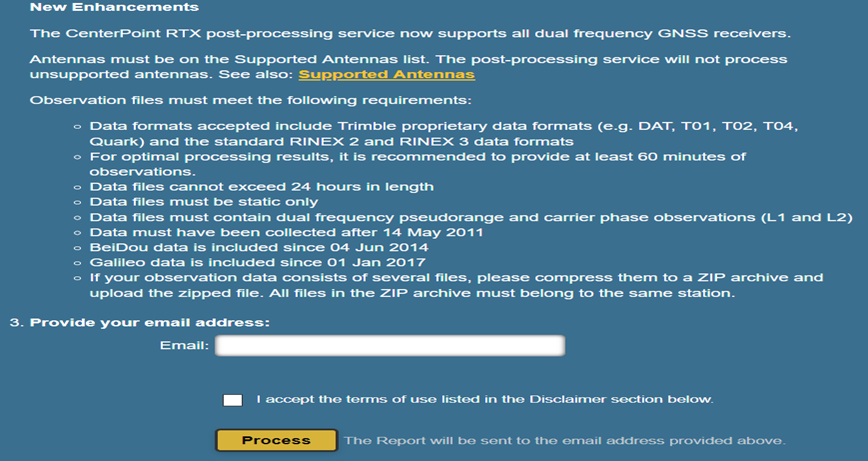
\includegraphics[width=\linewidth]{images/pic06}
	\caption{Интерфейс сайта Trimble RTX}
	\label{fig:pic06}
\end{figure}

При обработке с использованием данного интернет-сервиса необходимо загрузить обрабатываемый RINEX-файл либо фирменный формат Trimble (T01, T02, T03, T04). Далее выбирается литосферная плита, либо указывается автоматически в процессе обработки. Затем указывается электронная почта, на которую придет обработанный файл в формате pdf. На рисунке \cref{fig:pic07} приведен пример отчета по обработке с использованием данного интернет-сервиса.

\begin{figure}[h]
	\centering
	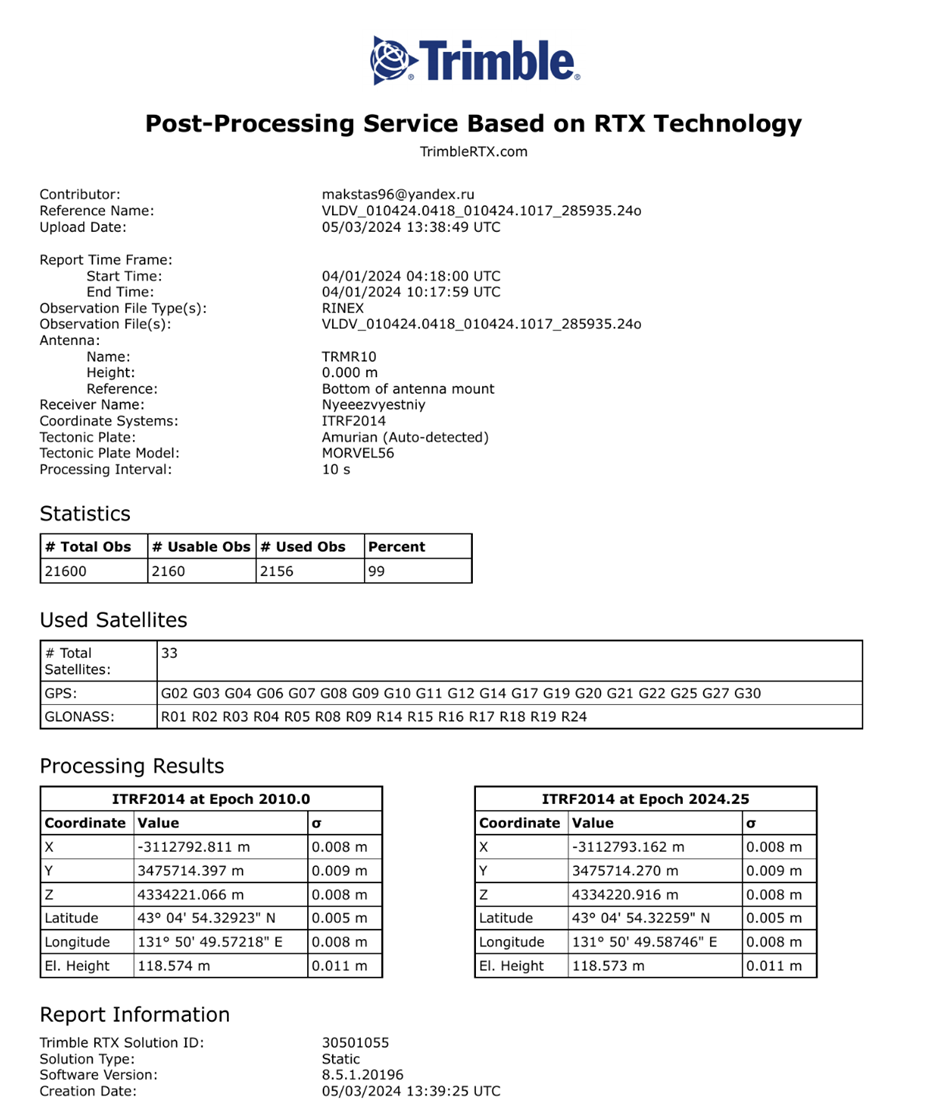
\includegraphics[width=\linewidth]{images/pic07}
	\caption{Пример отчета Trimble RTX}
	\label{fig:pic07}
\end{figure}

Как видно из рисунка \cref{fig:pic07} в отчете указывается вся интересующая информация: время начала и окончания измерения; количество используемых ГНСС и номер спутников; и координаты, приводимые на 2 эпохи в двух представлениях. В геодезической системе координат(BLH) и геоцентрической(XYZ). 

\subsection{Magic PPP (magic GNNS)}\label{subsec:ch2/sec1/sub2}

Magic PPP --- это глобальный сервис позиционирования, который позволяет пользователям GNSS определять своё положение или траекторию с сантиметровой точностью. 

Метод, используемый в magic PPP, не требует данных от непрерывных опорных станций (CORS), работающих в непосредственной близости от приемника. Идеальное решение для точной траектографии на больших расстояниях и/или в областях, отличных от покрытия CORS.

Данный сервис состоит из 4-х служб-составляющих. С более подробной информацией можно ознакомиться на официальном сайте \cite{src69}. 
 
 
\subsection{Canadian Spatial Reference System (CSRS-PPP)  }\label{subsec:ch2/sec1/sub3}
 
CSRS – Канадский сервис, предназначенный для обработки спутниковых данных по РРР-алгоритму.
 
Основные сведения о сервисе: 
 
\begin{list}{$ \checkmark $\\[6pt]} {\parsep = \parskip \itemsep=\parsep \topsep=0em}
	\item Бесплатный сервис. 
	\item Присутствует возможность обработки любых форматов сырых данных, собранных ГНСС-аппаратурой.
	\item Возможно, обрабатывать как статические, так и кинематические данные.
	\item Возможна загрузка как данных, собранных двухчастотным, так и одночастотным приемником.
\end{list}

В отличии от интернет-сервиса Trimble RTX у данного сервиса реализована обработка как статических, так и кинематических данных. 

Результаты обработки могут быть представлены как в системе координат ITRF, так и в локальной системе координат, применяемой на территории Северной Америки --- NAD-83. В \textbf{\underline{приложении F}} приведен отчет с данного интернет-сервиса.


\subsection{Automatic Precise Points Positioning Service (APPS)}\label{subsec:ch2/sec1/sub4}

APPS принимает файлы GPS-измерений и применяет самую передовую технологию GPS-позиционирования из Лаборатории реактивного движения NASA для оценки положения ваших GPS-приемников, независимо от того, находятся ли они в статике, в движении, на земле или в воздухе \cite{src80}.

Основные сведения о APPS:

\begin{list}{$ \checkmark $\\[6pt]} {\parsep = \parskip \itemsep=\parsep \topsep=0em}
	\item Бортовые эфемериды и поправки к часам в режиме реального времени GPS~JPL. 
	\item Уточненные и высокоточные (фиальные) эфемериды от JPL.
	\item Инернет-сервис и программное обеспечение  GIPSY-OASIS содержит один и тот же алгоритм.
	\item Поддерживает форматы данных: RINEX~2, RINEX~2.11 и фирменный формат данных GPSY~TDP.
\end{list}

\subsection{GNSS Analysis and Positioning Software (GAPS)}\label{subsec:ch2/sec1/sub5}

GAPS обеспечивает пользователям точное позиционирование с использованием одного спутникового приемника геодезического класса как в статическом, так и в кинематическом режиме. Благодаря использованию высокоточных эфемерид и поправок к часам, предоставляемых такими источниками, как Международная служба ГНСС (IGS) и Natural Resources Canada (NRCan), можно легко достичь точность на сантиметровом уровне в статическом режиме и позиционирования на дециметровом уровне в кинематическом режиме при достаточной продолжительности измерения.

\subsection{OPUS}\label{subsec:ch2/sec1/sub6}

Этот сервис предназначен для обработки спутниковых данных с использованием РРР-алгоритма. Он обеспечивает простой доступ к высокоточным координатам Национальной пространственной системы отсчета NSRS.  Для успешной реализации необходимо загрузить исходный файл, а обработанные координаты придут на указанную электронную почту.

OPUS требует минимального пользовательского ввода и обработка происходит с использованием программного обеспечения, которое вычисляет координаты для сетей NGS Continuous Operating Reference Station (далее «CORS»). 

У данного интернет-сервиса есть ряд требований, предъявляемых к сырым файлам:

\begin{list}{$ \checkmark $\\[6pt]} {\parsep = \parskip \itemsep=\parsep \topsep=0em}
	\item Данные должны быть собраны двухчастотным спутниковым приемником. 
	\item Возможно обрабатывать данные продолжительностью измерений начиная с 15 минут и заканчивая 48 часами.
	\item Файлы продолжительностью менее двух часов обязательно должны содержать не только P2, но и P1 или C1.
	\item Частота записи может быть 1,2,3,5,10,15,30 секунд.
	\item Необходимо правильно выбирать антенну и высоту антенны. Неправильно выбранный тип антенны может выдать ошибку измерений в плане до 1~см; по высоте до 80~см.
\end{list}

\subsection{SOPAC SCOUT (Scripps Coordinate Update Tool of Scripps Orbit and Permanent Array Centre)}\label{subsec:ch2/sec1/sub7}

В основе сервиса SOPAC SCOUT лежит тот же принцип, что и в остальных интернет-сервисах. Однако в сравнении с другими сервисами есть пару ключевых отличий:

\begin{list}{$ \checkmark $\\[6pt]} {\parsep = \parskip \itemsep=\parsep \topsep=0em}
	\item Можно обрабатывать не более 10 проектов одновременно. 
	\item Минимальная рекомендуемая продолжительность измерений --- 1 час.
\end{list}


\subsection{IBGE-PPP (Scripps Coordinate Update Tool of Scripps Orbit and Permanent Array Centre)}\label{subsec:ch2/sec1/sub8}

Интернет-сервис был разработан Бразильским институтом географии и статистики. При этом, как и в случае интернет-сервисов Trimble RTX и CRSR количество одновременно обрабатываемых RINEX-файлов не ограничено.


\subsection{IGN-PPP}\label{subsec:ch2/sec1/sub9}

Данный интернет-сервис был разработан Аргентинским научным сообществом. В основе данного сервиса лежит интернет сервис CSRS. В \textbf{\underline{приложении Б}} приведен отчёт данного интернет-сервиса.


\subsection{PPP AS A SERVICE}\label{subsec:ch2/sec1/su10}

Интернет-сервис был разработан российским научным сообществом. PAAS (PPP as a service) обеспечивает возможность быстрого расчёта. В \textbf{\underline{приложении В}} приведен отчёт данного интернет-сервиса.


\subsection{Сравнение интернет-сервисов между собой}\label{subsec:ch2/sec1/sub11}

С целью сравнения интернет-сервисов между собой была создана таблица \cref{tab:tab03}, в которой приведены основные сравнительные характеристики. Для компактной записи были использованы общепринятые обозначения R -- ГЛОНАСС, G -- GPS.


\noindent\begin{minipage}{\linewidth}
	\centering\vspace{5mm}
	\captionof{table}{Сравнение данных между собой}\label{tab:tab03}\resizebox{\linewidth}{!}{%
		\begin{tabular}{|c|c|c|c|c|c|c|c|}
			\hline
			\textbf{Критерий} & \textbf{RTX} & \textbf{CRSR} & \begin{tabular}[c]{@{}l@{}}\textbf{Magic}\\ \textbf{GNNS}\end{tabular} & \textbf{GAPS} & \textbf{APPS} & \textbf{OPUS} & \textbf{PAAS} \\
			\hline
			\textbf{Дискретность} & все & $\ge30$ сек. & все & все & все & все & все \\
			\hline
			\textbf{СК} & BLH, ITRF & \begin{tabular}[c]{@{}l@{}}BLH, NAD,\\ \ \ \ \ ITRF\end{tabular} & BLH, ITRF & BLH, ITRF & BLH, ITRF & \begin{tabular}[c]{@{}l@{}}BLH, ITRF,\\ \ \ \ \ \ \ UTM\end{tabular} &  \\
			\hline
			\textbf{$\mathbf{t_{min}}$ (мин)} & $10$ & $10$ & $10$ & $10$ & $10$ & $15$ &  \\
			\hline
			\textbf{$\mathbf{t_{max}}$ (ч)} & $24$ & $24$ & $24$ & $24$ & $24$ & $24$ &  \\
			\hline
			\textbf{$\mathbf{t_\text{обработки}}$ (мин)} & $2-3$ & $2-3$ & $4$ & $10-15$ & $5$ & $5$ & $3$ \\
			\hline
			\begin{tabular}[c]{@{}l@{}}\textbf{ \ \ \ ГНСС}\\\textbf{комбинации} \end{tabular} & R, G, C & R, G & R, G & R, G & R, G & R, G & R, G \\
			\hline
			\begin{tabular}[c]{@{}l@{}}\textbf{Количество}\\\textbf{ \ проектов}\end{tabular} & $\infty$ & $\infty$ & $\infty$ & $\infty$ & $\infty$ & $\infty$ &  \\
			\hline
		\end{tabular}
	}
\end{minipage}\vspace{5mm}


Из таблицы \cref{tab:tab03} видно, что с точки зрения времени, затрачиваемого на обработку измерений, быстрее происходит предоставление результатов в случае использования RTX и CRSR. Однако у CRSR обработка данных выполняется только при периодичности записи 30 секунд и реже. Конечно, можно использовать и более высокую частоту, но в таком случае данные будут прорежены, что может привести к существенному снижению точности получаемого решения. Также можно заключить, что интернет-сервис SOPAC SCOUT выполняет работу медленнее прочих.



\section{Обзор современных программных обеспечений для обработки РРР}\label{sec:ch2/sec2}

\subsection{Bernese} \label{subsec:ch2/sec2/sub1}

Программное обучение Bernese было разработано в астрономическом институте Бернского университета для постобработки наблюдений GNSS в научных исследованиях \cite{src47}. Это программное обеспечение используется Европейским орбитальным центром (Code) для поддержки международных (IGS) и европейских (EUREF/EPN) глобальных спутниковых навигационных сетей. 

В программном обеспечении можно обрабатывать как статические, так и кинематические наблюдения. Помимо этого, используя программное обеспечение Bernese существует возможность обрабатывать данные в результате высокоточного позиционирования (РРР). Благодаря встроенным моделям существует возможность учитывать движение литосферных плит, грунтов, а также приливы и отливы. К тому же постоянно поддерживается учет зенитной тропосферной задержки и градиента, параметров ориентации Земли и глобальных ионосферных моделей \cite{src51,src52}.

\subsection{GIPSY-OASIS} \label{subsec:ch2/sec2/sub2}

Лаборатория реактивного движения Национального управления по аэронавтике и исследованию космического пространства (НАСА) в Пасадене, штат Калифорния, обеспечивает поддержку пользователей GIPSY-OASIS (GOA II) --- автоматизированного, быстрого, сверхточного программного комплекса для обработки высокоточных данных GPS со строгим контролем качества данных.

\subsection{Waypoint Grafnet} \label{subsec:ch2/sec2/sub3}

Программное обеспечение для постобработки Graphnet --- это мощный программный комплекс, для обеспечения наилучшей статической или кинематической точности ГНСС с использованием всех доступных данных ГНСС. Поддержка форматов данных для большинства одно- и многочастотных коммерческих приемников означает, что Graphnav, скорее всего, будет работать с существующим оборудованием \cite{src67}.

\subsection{RTKLIB} \label{subsec:ch2/sec2/sub4}

RTKLIB --- набор библиотек с открытым кодом. Данное программное обеспечение предназначено для обработки как статических, так и кинематических данных \cite{src72}. Среди преимуществ данного программного обеспечения стоит выделить возможность обработки данных только ГЛОНАСС, что ни в одном другом программном обеспечении или интернет-сервисе не реализовано.  

\subsection{КРЕДО ГНСС} \label{subsec:ch2/sec2/sub5}

В программном обеспечении КРЕДО ГНСС присутствует возможность обработки спутниковых данных не только по стандартным алгоритмам, но и при использовании методов высокоточных координатных определений. Данная возможность появилась с выходом версии 2.0.

\subsection{Trimble Business Centre}\label{subsec:ch2/sec2/sub6}

В современных версиях программного обеспечения Trimble Bisiness Centre (далее «TBC») присутствует возможность не только обработки спутниковых данных, но также данных с применением наземных методов, фотограмметрии и результатов лазерного сканирования. Кроме того в программном обеспечении реализована возможность обработки данных и по РРР-алгоритму \cite{src65,src67}.

\subsection{TropoGNSS}\label{subsec:ch2/sec2/sub7}

TropoGNSS --- программный продукт для мониторинга параметров атмосферы и движений земной коры, рассчитываемых по измерениям сигналов Глобальных Навигационных Спутниковых Систем (ГНСС). Данное приложение разработано в Казанском федеральном университете и является одним из немногих примеров российских научных программных продуктов в этой сфере. В TropoGNSS реализован абсолютный метод обработки данных ГНСС, называемый технологией PPP (Precise Point Positioning). Эта технология предполагает получение высокоточных результатов по данным одиночной станции. Применяемый в программе алгоритм основан на сравнении длин геометрического и фазового пути радиоволн от спутников ГНСС до наземного приемника. Уравнивание измерений производится с помощью фильтра Калмана. В настоящее время приложение поддерживает обработку данных американской системы GPS, российской системы ГЛОНАСС и европейской системы Galileo.

\subsection{ПроГеоСеть}\label{subsec:ch2/sec2/sub8}

ПроГеоСеть современный программный продукт, представленный разработчиками в январе 2024 года. По заявлению разработчика (НИИ Микроэлектронной аппаратуры Прогресс) программное обеспечение является частью геодезического комплекса ПРОГЕО. По заявлению разработчиков данное программное обеспечение предназначено для: позиционирования и навигации статических и подвижных объектов на основе данных спутниковых систем GPS, ГЛОНАСС, Galileo, Beidou, QZSS, IRNSS методами RTK, RTPK, PPP и классической постобработкой \cite{src36}.

Помимо выше перечисленного, в настоящее время, по заявлению производителей, программное обеспечение происходит процедуру сертификации и в геодезическом производстве \textbf{\textit{будет использоваться с середины 2024 года}}.


\section{Исследование точности определения координат, при использовании современных способов обработки данных по РРР-алгоритму}\label{sec:ch2/sec3}

Полевые экспериментальные работы выполнялись с 21.01.2022 по 14.02.2022 в общей сложности --- 12 дней по 3-5 часов ежедневно на крыше седьмого корпуса РУТ(МИИТ) с использованием двухчастотного спутникового приемника Trimble R10. На рисунке \cref{fig:pic08} представлен описываемый пункт (MIIT).

\begin{figure}[h]
	\centering
	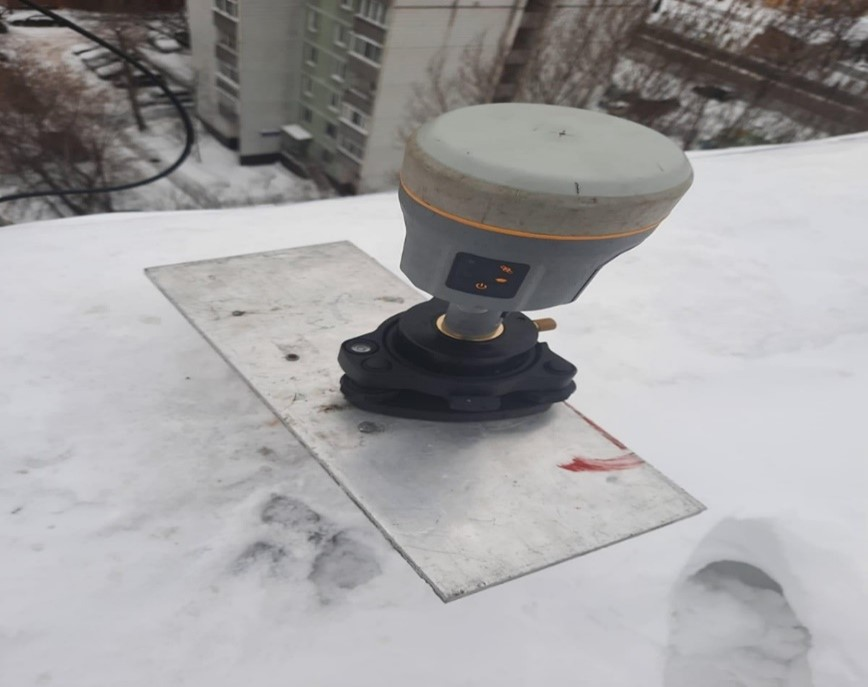
\includegraphics[width=0.7\linewidth]{images/pic08}
	\caption{Спутниковый приемник на крыше}
	\label{fig:pic08}
\end{figure}

Периодичность записи измерений составляла 10 секунд.  Среднее время проведения экспериментальных работ с 12:00 до 15:00. После проведения съёмочных работ сырые файлы преобразовывались в формат RINEX версии 2.11 с использованием программного обеспечения Trimble Convert to RINEX \cite{src84}. 

Для исследования точности обработки данных по РРР-алгоритму были поставлены следующие цели:

\begin{enumerate}
	\item Выявить влияние продолжительности измерений на данные, получаемые при обработке по РРР-алгоритму. 
	\item Выявить влияние количества принимаемых спутников и оценить влияние pdop фактора на получаемые результаты.
	\item Проанализировать точность при использовании ГНСС в различных комбинациях (только ГЛОНАСС; только GPS; совместно ГЛОНАСС и GPS).
	\item Рассмотреть получаемую точность при обработке многократных спутниковых измерений.
	\item Рассмотреть влияние частоты записи \textbf{на получаемые приращения координат}.
	\item Произвести сравнение между реализациями с использованием программных обеспечений и интернет-сервисов.
\end{enumerate}

Этапы проведения работ и полученные результаты приведены в пунктах \cref{subsec:ch2/sec3/sub1}, \cref{subsec:ch2/sec3/sub2}, \cref{subsec:ch2/sec3/sub3}, \cref{subsec:ch2/sec3/sub4}, \cref{subsec:ch2/sec3/sub5}.




\subsection[Влияние многократных измерений]{Исследование точности при многократных спутниковых измерениях}\label{subsec:ch2/sec3/sub1}

Для исследования координат, определяемых по РРР-алгоритму \textit{с точки зрения многократных измерений}, было выполнено следующее:
%были подготовлены RINEX-файлы, содержащие одно-, двух- и трёхчасовые интервалы измерений.
\begin{enumerate}
	\item Были подготовлены RINEX-файлы, содержащие трёхчасовые интервалы измерений. 
	\item Впоследствии RINEX-файлы были преобразованы в наборы данных, содержащие одно-, двух- и трёхчасовые интервалы.
\end{enumerate}

\subsubsection{Обработка с использованием интернет-сервиса Trimble RTX }\label{subsec:ch2/sec3/sub1/sub1}

Обработка данных РРР-алгоритмом по RTX обработке, производится на сайте Trimble-RTX \cite{src44}. Обработка выполняется автоматически после загрузки RINEX-файла. По её завершении можно скачать результаты.

Этот процесс повторяется последовательно ко всем RINEX-файлам. Ниже, в таблице \cref{tab:tab04}, приведены координаты пункта (MIIT), полученные из \textit{одночасовых} измерений, выполнявшихся в течение двенадцати дней.

\begin{table} [h!]
	\centering\small
	\captionof{table}{Координаты пункта MIIT. Сервис Trimble RTX, $T_{\text{изм.}}=1$ час}\label{tab:tab04}{%
		\begin{tabular}{|c|c|c|c|c|}
			\hline
			\textbf{№} & \textbf{Дата} & \textbf{X, м} & \textbf{Y, м} & \textbf{Z, м} \\
			\hline
			\textbf{ $\mathbf{1}$} & $21.01.2022$ & $2847750,924$ & $2193184,486$ & $5251441,725$ \\
			\hline
			\textbf{ $\mathbf{2}$} & $26.01.2022$ & $2847750,932$ & $2193184,486$ & $5251441,735$ \\
			\hline
			\textbf{ $\mathbf{3}$} & $27.01.2022$ & $2847750,927$ & $2193184,487$ & $5251441,733$ \\
			\hline
			\textbf{ $\mathbf{4}$} & $28.01.2022$ & $2847750,934$ & $2193184,486$ & $5251441,737$ \\
			\hline
			\textbf{ $\mathbf{5}$} & $31.01.2022$ & $2847750,945$ & $2193184,494$ & $5251441,735$ \\
			\hline
			\textbf{ $\mathbf{6}$} & $01.02.2022$ & $2847750,927$ & $2193184,475$ & $5251441,703$ \\
			\hline
			\textbf{ $\mathbf{7}$} & $02.02.2022$ & $2847750,931$ & $2193184,483$ & $5251441,730$ \\
			\hline
			\textbf{ $\mathbf{8}$} & $03.02.2022$ & $2847750,933$ & $2193184,483$ & $5251441,725$ \\
			\hline
			\textbf{ $\mathbf{9}$} & $04.02.2022$ & $2847750,933$ & $2193184,481$ & $5251441,723$ \\
			\hline
			\textbf{$\mathbf{10}$} & $09.02.2022$ & $2847750,930$ & $2193184,488$ & $5251441,733$ \\
			\hline
			\textbf{$\mathbf{11}$} & $10.02.2022$ & $2847750,934$ & $2193184,491$ & $5251441,740$ \\
			\hline
			\textbf{$\mathbf{12}$} & $14.02.2022$ & $2847750,946$ & $2193184,496$ & $5251441,736$ \\
			\hline
		\end{tabular}
	}
\end{table}

В таблице \cref{tab:tab05} приведены координаты пункта (MIIT), полученные из \textit{двухчасовых} измерений, выполнявшихся в течение двенадцати дней.

\begin{table} [htbp]
	\centering\small
	\captionof{table}{Координаты пункта MIIT. Сервис Trimble RTX, $T_{\text{изм.}}=2$ часа}\label{tab:tab05}{%
		\begin{tabular}{|c|c|c|c|c|}
			\hline
			\textbf{№} & \textbf{Дата} & \textbf{X, м} & \textbf{Y, м} & \textbf{Z, м} \\
			\hline
			\textbf{ $\mathbf{1}$} & $21.01.2022$ & $2847750,925$ & $2193184,483$ & $5251441,713$ \\
			\hline
			\textbf{ $\mathbf{2}$} & $26.01.2022$ & $2847750,928$ & $2193184,487$ & $5251441,722$ \\
			\hline
			\textbf{ $\mathbf{3}$} & $27.01.2022$ & $2847750,930$ & $2193184,487$ & $5251441,723$ \\
			\hline
			\textbf{ $\mathbf{4}$} & $28.01.2022$ & $2847750,937$ & $2193184,491$ & $5251441,733$ \\
			\hline
			\textbf{ $\mathbf{5}$} & $31.01.2022$ & $2847750,941$ & $2193184,496$ & $5251441,737$ \\
			\hline
			\textbf{ $\mathbf{6}$} & $01.02.2022$ & $2847750,932$ & $2193184,488$ & $5251441,722$ \\
			\hline
			\textbf{ $\mathbf{7}$} & $02.02.2022$ & $2847750,937$ & $2193184,492$ & $5251441,736$ \\
			\hline
			\textbf{ $\mathbf{8}$} & $03.02.2022$ & $2847750,934$ & $2193184,492$ & $5251441,728$ \\
			\hline
			\textbf{ $\mathbf{9}$} & $04.02.2022$ & $2847750,938$ & $2193184,490$ & $5251441,734$ \\
			\hline
			\textbf{$\mathbf{10}$} & $09.02.2022$ & $2847750,933$ & $2193184,491$ & $5251441,729$ \\
			\hline
			\textbf{$\mathbf{11}$} & $10.02.2022$ & $2847750,932$ & $2193184,487$ & $5251441,725$ \\
			\hline
			\textbf{$\mathbf{12}$} & $14.02.2022$ & $2847750,939$ & $2193184,490$ & $5251441,728$ \\
			\hline
		\end{tabular}
	}
\end{table}

В таблице \cref{tab:tab06} приведены координаты пункта (MIIT), полученные из \textit{трёхчасовых} измерений выполнявшихся в течение двенадцати дней.

\begin{table} [htbp]
	\centering\small
	\captionof{table}{Координаты пункта MIIT. Сервис Trimble RTX, $T_{\text{изм.}}=3$ часа}\label{tab:tab06}{%
		\begin{tabular}{|c|c|c|c|c|}
			\hline
			\textbf{№} & \textbf{Дата} & \textbf{X, м} & \textbf{Y, м} & \textbf{Z, м} \\
			\hline
			\textbf{ $\mathbf{1}$} & $21.01.2022$ & $2847750,927$ & $2193184,485$ & $5251441,714$ \\
			\hline
			\textbf{ $\mathbf{2}$} & $26.01.2022$ & $2847750,932$ & $2193184,489$ & $5251441,724$ \\
			\hline
			\textbf{ $\mathbf{3}$} & $27.01.2022$ & $2847750,933$ & $2193184,488$ & $5251441,724$ \\
			\hline
			\textbf{ $\mathbf{4}$} & $28.01.2022$ & $2847750,939$ & $2193184,493$ & $5251441,734$ \\
			\hline
			\textbf{ $\mathbf{5}$} & $31.01.2022$ & $2847750,943$ & $2193184,497$ & $5251441,736$ \\
			\hline
			\textbf{ $\mathbf{6}$} & $01.02.2022$ & $2847750,933$ & $2193184,488$ & $5251441,723$ \\
			\hline
			\textbf{ $\mathbf{7}$} & $02.02.2022$ & $2847750,937$ & $2193184,491$ & $5251441,732$ \\
			\hline
			\textbf{ $\mathbf{8}$} & $03.02.2022$ & $2847750,933$ & $2193184,489$ & $5251441,721$ \\
			\hline
			\textbf{ $\mathbf{9}$} & $04.02.2022$ & $2847750,940$ & $2193184,489$ & $5251441,727$ \\
			\hline
			\textbf{$\mathbf{10}$} & $09.02.2022$ & $2847750,931$ & $2193184,486$ & $5251441,721$ \\
			\hline
			\textbf{$\mathbf{11}$} & $10.02.2022$ & $2847750,932$ & $2193184,485$ & $5251441,721$ \\
			\hline
			\textbf{$\mathbf{12}$} & $14.02.2022$ & $2847750,938$ & $2193184,489$ & $5251441,723$ \\
			\hline
		\end{tabular}
	}
\end{table}

В дальнейшем были найдены разности приращений координат между вычисленными и усредненными координатами, сведёнными в таблицу \cref{tab:tab07}. 
Значения усредненных координат: 
$$
	\left\{
	\begin{matrix}
		\overline{X} = 2847750,943 \pm 000,000 \text{ м}, \\
		\overline{Y} = 2193184,497 \pm 000,000 \text{ м}, \\
		\overline{Z} = 5251441,736 \pm 000,000 \text{ м.}
	\end{matrix}
	\right.
$$

\begin{table} [htbp]
	\centering\small
	\captionof{table}{Разности координат. Сервис Trimble RTX}\label{tab:tab07}{%
		\begin{tabular}{|c|rrr|rrr|rrr|}
			\hline
			\multirow{2}{*}{\textbf{№}} & 
			\multicolumn{3}{c|}{\textbf{1 час}}                                                                             & \multicolumn{3}{c|}{\textbf{2 часа}}                                                                            & \multicolumn{3}{c|}{\textbf{3 часа}}                                                                            \\ \cline{2-10} 
			& \multicolumn{1}{l|}{\textbf{σX, м}} & \multicolumn{1}{l|}{\textbf{σY, м}} & \multicolumn{1}{l|}{\textbf{σZ, м}} & \multicolumn{1}{l|}{\textbf{σX, м}} & \multicolumn{1}{l|}{\textbf{σY, м}} & \multicolumn{1}{l|}{\textbf{σZ, м}} & \multicolumn{1}{l|}{\textbf{σX, м}} & \multicolumn{1}{l|}{\textbf{σY, м}} & \multicolumn{1}{l|}{\textbf{σZ, м}} \\ \hline
			\textbf{1}                  & 
			\multicolumn{1}{r|}{$ 0,019$}       & \multicolumn{1}{r|}{$-0,011$}       & $-0,011$                            & \multicolumn{1}{r|}{$ 0,018$}       & \multicolumn{1}{r|}{$-0,014$}       & $-0,023$                            & \multicolumn{1}{r|}{$ 0,016$}       & \multicolumn{1}{r|}{$-0,012$}       & $-0,022$                            \\ \hline
			\textbf{2}                  & 
			\multicolumn{1}{r|}{$-0,011$}       & \multicolumn{1}{r|}{$-0,011$}       & $-0,001$                            & \multicolumn{1}{r|}{$-0,015$}       & \multicolumn{1}{r|}{$-0,010$}       & $-0,014$                            & \multicolumn{1}{r|}{$-0,011$}       & \multicolumn{1}{r|}{$-0,008$}       & $-0,012$                            \\ \hline
			\textbf{3}                  & 
			\multicolumn{1}{r|}{$-0,016$}       & \multicolumn{1}{r|}{$-0,010$}       & $-0,003$                            & \multicolumn{1}{r|}{$-0,013$}       & \multicolumn{1}{r|}{$-0,010$}       & $-0,013$                            & \multicolumn{1}{r|}{$-0,010$}       & \multicolumn{1}{r|}{$-0,009$}       & $-0,012$                            \\ \hline
			\textbf{4}                  & 
			\multicolumn{1}{r|}{$-0,019$}        & \multicolumn{1}{r|}{$-0,011$}       & $-0,011$                            & \multicolumn{1}{r|}{$-0,018$}        & \multicolumn{1}{r|}{$-0,014$}       & $-0,023$                            & \multicolumn{1}{r|}{$-0,016$}        & \multicolumn{1}{r|}{$-0,012$}       & $-0,022$                            \\ \hline
			\textbf{5}                  & 
			\multicolumn{1}{r|}{$-0,011$}        & \multicolumn{1}{r|}{$-0,011$}       & $-0,001$                            & \multicolumn{1}{r|}{$-0,015$}        & \multicolumn{1}{r|}{$-0,010$}       & $-0,014$                            & \multicolumn{1}{r|}{$-0,011$}        & \multicolumn{1}{r|}{$-0,008$}       & $-0,012$                            \\ \hline
			\textbf{6}                  & 
			\multicolumn{1}{r|}{$-0,016$}        & \multicolumn{1}{r|}{$-0,010$}       & $-0,003$                            & \multicolumn{1}{r|}{$-0,013$}        & \multicolumn{1}{r|}{$-0,010$}       & $-0,013$                            & \multicolumn{1}{r|}{$-0,010$}        & \multicolumn{1}{r|}{$-0,009$}       & $-0,012$                            \\ \hline
			\textbf{7}                  & 
			\multicolumn{1}{r|}{$ 0,012$}        & \multicolumn{1}{r|}{$-0,014$}       & $-0,006$                            & \multicolumn{1}{r|}{$ 0,006$}        & \multicolumn{1}{r|}{$-0,005$}       & $ 0,000$                            & \multicolumn{1}{r|}{$ 0,006$}        & \multicolumn{1}{r|}{$-0,006$}       & $-0,004$                            \\ \hline
			\textbf{8}                  & 
			\multicolumn{1}{r|}{$-0,010$}        & \multicolumn{1}{r|}{$-0,014$}       & $-0,011$                            & \multicolumn{1}{r|}{$-0,009$}        & \multicolumn{1}{r|}{$-0,005$}       & $-0,008$                            & \multicolumn{1}{r|}{$-0,010$}        & \multicolumn{1}{r|}{$-0,008$}       & $-0,015$                            \\ \hline
			\textbf{9}                  & 
			\multicolumn{1}{r|}{$-0,010$}        & \multicolumn{1}{r|}{$-0,016$}       & $-0,013$                            & \multicolumn{1}{r|}{$-0,005$}        & \multicolumn{1}{r|}{$-0,007$}       & $-0,002$                            & \multicolumn{1}{r|}{$-0,003$}        & \multicolumn{1}{r|}{$-0,008$}       & $-0,009$                            \\ \hline
			\textbf{10}                 & 
			\multicolumn{1}{r|}{$-0,013$}        & \multicolumn{1}{r|}{$-0,009$}       & $-0,003$                            & \multicolumn{1}{r|}{$-0,010$}        & \multicolumn{1}{r|}{$-0,006$}       & $-0,007$                            & \multicolumn{1}{r|}{$-0,012$}        & \multicolumn{1}{r|}{$-0,011$}       & $-0,015$                            \\ \hline
			\textbf{11}                 & 
			\multicolumn{1}{r|}{$-0,009$}        & \multicolumn{1}{r|}{$-0,006$}       & $ 0,004$                            & \multicolumn{1}{r|}{$-0,011$}        & \multicolumn{1}{r|}{$-0,010$}       & $-0,011$                            & \multicolumn{1}{r|}{$-0,011$}        & \multicolumn{1}{r|}{$-0,012$}       & $-0,015$                            \\ \hline
			\textbf{12}                 & 
			\multicolumn{1}{r|}{$ 0,003$}        & \multicolumn{1}{r|}{$-0,001$}       & $ 0,000$                            & \multicolumn{1}{r|}{$-0,004$}        & \multicolumn{1}{r|}{$-0,007$}       & $-0,008$                            & \multicolumn{1}{r|}{$-0,005$}        & \multicolumn{1}{r|}{$-0,008$}       & $-0,013$                            \\ \hline
		\end{tabular}
	}
\end{table}


В таблице \cref{tab:tab08} приводятся средние, а также минимальные и максимальные значения разностей координат.

\begin{table} [htbp]
	\centering\small
	\captionof{table}{Обобщённые разности координат. Сервис Trimble RTX}\label{tab:tab08}{%\resizebox{\linewidth}{!}{%
		\begin{tabular}{|c|rrr|rrr|rrr|}
			\hline
			\multirow{2}{*}{\textbf{ }} & 
			\multicolumn{3}{c|}{\textbf{1 час}}  & \multicolumn{3}{c|}{\textbf{2 часа}}  & \multicolumn{3}{c|}{\textbf{3 часа}}  \\ \cline{2-10} & 
			\multicolumn{1}{l|}{\textbf{σX, м}} & \multicolumn{1}{l|}{\textbf{σY, м}} & \multicolumn{1}{l|}{\textbf{σZ, м}} & \multicolumn{1}{l|}{\textbf{σX, м}} & \multicolumn{1}{l|}{\textbf{σY, м}} & \multicolumn{1}{l|}{\textbf{σZ, м}} & \multicolumn{1}{l|}{\textbf{σX, м}} & \multicolumn{1}{l|}{\textbf{σY, м}} & \multicolumn{1}{l|}{\textbf{σZ, м}} \\ \hline
			\textbf{мин.}                       & \multicolumn{1}{r|}{$-0,019$}       & \multicolumn{1}{r|}{$-0,022$}         & $-0,033$                            & \multicolumn{1}{r|}{$-0,018$}       & \multicolumn{1}{r|}{$-0,014$}         & $-0,023$                            & \multicolumn{1}{r|}{$-0,016$}       & \multicolumn{1}{r|}{$-0,012$}         & $-0,022$                              \\ \hline
			\textbf{макс.}                      & \multicolumn{1}{r|}{$0,003$}        & \multicolumn{1}{r|}{$-0,001$}         & $0,004$                             & \multicolumn{1}{r|}{$-0,002$}       & \multicolumn{1}{r|}{$-0,001$}         & $0,001$                             & \multicolumn{1}{r|}{$0,000$}        & \multicolumn{1}{r|}{$0,000$}          & $0,000$                              \\ \hline
			\textbf{среднее}                    & \multicolumn{1}{r|}{$-0,010$}       & \multicolumn{1}{r|}{$-0,011$}         & $-0,006$                            & \multicolumn{1}{r|}{$-0,009$}       & \multicolumn{1}{r|}{$-0,007$}         & $-0,008$                            & \multicolumn{1}{r|}{$-0,008$}       & \multicolumn{1}{r|}{$-0,008$}         & $-0,011$                              \\ \hline
		\end{tabular}
	}
\end{table}

Анализируя таблицу \cref{tab:tab08} можно заметить, что в среднем величины отклонений координат содержат одинаковую ошибку при 12-дневыных измерениях.




\subsubsection{Обработка с использованием интернет-сервиса CSRS }\label{subsec:ch2/sec3/sub1/sub2}


Обработка происходила интернет-сервисом CSRS. Был использован тот же набор RINEX-файлов данных. Этапы обработки те же самые. Результаты приведены в таблице \cref{tab:tab09}.


\begin{table} [htbp]
	\centering\small
	\captionof{table}{Разности координат. Сервис CSRS}\label{tab:tab09}{%
		\begin{tabular}{|c|rrr|rrr|rrr|}
			\hline
			\multirow{2}{*}{\textbf{№}} & 
			\multicolumn{3}{c|}{\textbf{1 час}}                                                                             & \multicolumn{3}{c|}{\textbf{2 часа}}                                                                            & \multicolumn{3}{c|}{\textbf{3 часа}}                                                                            \\ \cline{2-10} 
			& \multicolumn{1}{l|}{\textbf{σX, м}} & \multicolumn{1}{l|}{\textbf{σY, м}} & \multicolumn{1}{l|}{\textbf{σZ, м}} & \multicolumn{1}{l|}{\textbf{σX, м}} & \multicolumn{1}{l|}{\textbf{σY, м}} & \multicolumn{1}{l|}{\textbf{σZ, м}} & \multicolumn{1}{l|}{\textbf{σX, м}} & \multicolumn{1}{l|}{\textbf{σY, м}} & \multicolumn{1}{l|}{\textbf{σZ, м}} \\ \hline
			\textbf{1}                  & 
			\multicolumn{1}{r|}{$ 0,019$}       & \multicolumn{1}{r|}{$-0,011$}       & $-0,011$                            & \multicolumn{1}{r|}{$ 0,018$}       & \multicolumn{1}{r|}{$-0,014$}       & $-0,023$                            & \multicolumn{1}{r|}{$ 0,016$}       & \multicolumn{1}{r|}{$-0,012$}       & $-0,022$                            \\ \hline
			\textbf{2}                  & 
			\multicolumn{1}{r|}{$-0,011$}       & \multicolumn{1}{r|}{$-0,011$}       & $-0,001$                            & \multicolumn{1}{r|}{$-0,015$}       & \multicolumn{1}{r|}{$-0,010$}       & $-0,014$                            & \multicolumn{1}{r|}{$-0,011$}       & \multicolumn{1}{r|}{$-0,008$}       & $-0,012$                            \\ \hline
			\textbf{3}                  & 
			\multicolumn{1}{r|}{$-0,016$}       & \multicolumn{1}{r|}{$-0,010$}       & $-0,003$                            & \multicolumn{1}{r|}{$-0,013$}       & \multicolumn{1}{r|}{$-0,010$}       & $-0,013$                            & \multicolumn{1}{r|}{$-0,010$}       & \multicolumn{1}{r|}{$-0,009$}       & $-0,012$                            \\ \hline
			\textbf{4}                  & 
			\multicolumn{1}{r|}{$-0,019$}       & \multicolumn{1}{r|}{$-0,011$}       & $-0,011$                            & \multicolumn{1}{r|}{$-0,018$}       & \multicolumn{1}{r|}{$-0,014$}       & $-0,023$                            & \multicolumn{1}{r|}{$-0,016$}       & \multicolumn{1}{r|}{$-0,012$}       & $-0,022$                            \\ \hline
			\textbf{5}                  & 
			\multicolumn{1}{r|}{$-0,011$}       & \multicolumn{1}{r|}{$-0,011$}       & $-0,001$                            & \multicolumn{1}{r|}{$-0,015$}       & \multicolumn{1}{r|}{$-0,010$}       & $-0,014$                            & \multicolumn{1}{r|}{$-0,011$}       & \multicolumn{1}{r|}{$-0,008$}       & $-0,012$                            \\ \hline
			\textbf{6}                  & 
			\multicolumn{1}{r|}{$-0,016$}       & \multicolumn{1}{r|}{$-0,010$}       & $-0,003$                            & \multicolumn{1}{r|}{$-0,013$}       & \multicolumn{1}{r|}{$-0,010$}       & $-0,013$                            & \multicolumn{1}{r|}{$-0,010$}       & \multicolumn{1}{r|}{$-0,009$}       & $-0,012$                            \\ \hline
			\textbf{7}                  & 
			\multicolumn{1}{r|}{$ 0,012$}       & \multicolumn{1}{r|}{$-0,014$}       & $-0,006$                            & \multicolumn{1}{r|}{$ 0,006$}       & \multicolumn{1}{r|}{$-0,005$}       & $ 0,000$                            & \multicolumn{1}{r|}{$ 0,006$}       & \multicolumn{1}{r|}{$-0,006$}       & $-0,004$                            \\ \hline
			\textbf{8}                  & 
			\multicolumn{1}{r|}{$-0,010$}       & \multicolumn{1}{r|}{$-0,014$}       & $-0,011$                            & \multicolumn{1}{r|}{$-0,009$}       & \multicolumn{1}{r|}{$-0,005$}       & $-0,008$                            & \multicolumn{1}{r|}{$-0,010$}       & \multicolumn{1}{r|}{$-0,008$}       & $-0,015$                            \\ \hline
			\textbf{9}                  & 
			\multicolumn{1}{r|}{$-0,010$}       & \multicolumn{1}{r|}{$-0,016$}       & $-0,013$                            & \multicolumn{1}{r|}{$-0,005$}       & \multicolumn{1}{r|}{$-0,007$}       & $-0,002$                            & \multicolumn{1}{r|}{$-0,003$}       & \multicolumn{1}{r|}{$-0,008$}       & $-0,009$                            \\ \hline
			\textbf{10}                 & 
			\multicolumn{1}{r|}{$-0,013$}       & \multicolumn{1}{r|}{$-0,009$}       & $-0,003$                            & \multicolumn{1}{r|}{$-0,010$}       & \multicolumn{1}{r|}{$-0,006$}       & $-0,007$                            & \multicolumn{1}{r|}{$-0,012$}       & \multicolumn{1}{r|}{$-0,011$}       & $-0,015$                            \\ \hline
			\textbf{11}                 & 
			\multicolumn{1}{r|}{$-0,009$}       & \multicolumn{1}{r|}{$-0,006$}       & $ 0,004$                            & \multicolumn{1}{r|}{$-0,011$}       & \multicolumn{1}{r|}{$-0,010$}       & $-0,011$                            & \multicolumn{1}{r|}{$-0,011$}       & \multicolumn{1}{r|}{$-0,012$}       & $-0,015$                            \\ \hline
			\textbf{12}                 & 
			\multicolumn{1}{r|}{$ 0,003$}       & \multicolumn{1}{r|}{$-0,001$}       & $ 0,000$                            & \multicolumn{1}{r|}{$-0,004$}       & \multicolumn{1}{r|}{$-0,007$}       & $-0,008$                            & \multicolumn{1}{r|}{$-0,005$}       & \multicolumn{1}{r|}{$-0,008$}       & $-0,013$                            \\ \hline
		\end{tabular}
	}
\end{table}

Основываясь на таблице \cref{tab:tab09} была создана таблица \cref{tab:tab10}, в которой указываются максимальные, минимальные и средние разности координат.


\begin{table} [htbp]
	\centering\small
	\captionof{table}{Обобщённые разности координат. Сервис CSRS}\label{tab:tab10}{%\resizebox{\linewidth}{!}{%
		\begin{tabular}{|c|rrr|rrr|rrr|}
			\hline
			\multirow{2}{*}{\textbf{ }} & 
			\multicolumn{3}{c|}{\textbf{1 час}}  & \multicolumn{3}{c|}{\textbf{2 часа}}  & \multicolumn{3}{c|}{\textbf{3 часа}}  \\ \cline{2-10} & 
			\multicolumn{1}{l|}{\textbf{σX, м}} & \multicolumn{1}{l|}{\textbf{σY, м}} & \multicolumn{1}{l|}{\textbf{σZ, м}} & \multicolumn{1}{l|}{\textbf{σX, м}} & \multicolumn{1}{l|}{\textbf{σY, м}} & \multicolumn{1}{l|}{\textbf{σZ, м}} & \multicolumn{1}{l|}{\textbf{σX, м}} & \multicolumn{1}{l|}{\textbf{σY, м}} & \multicolumn{1}{l|}{\textbf{σZ, м}} \\ \hline
			\textbf{мин.}                    & 
			\multicolumn{1}{r|}{$-0,022$}       & \multicolumn{1}{r|}{$-0,014$}         & $-0,027$                            & \multicolumn{1}{r|}{$-0,026$}       & \multicolumn{1}{r|}{$-0,006$}         & $-0,022$                            & \multicolumn{1}{r|}{$-0,025$}       & \multicolumn{1}{r|}{$-0,011$}         & $-0,027$                            \\ \hline
			\textbf{макс.}                   & 
			\multicolumn{1}{r|}{$-0,002$}       & \multicolumn{1}{r|}{$ 0,015$}         & $ 0,018$                            & \multicolumn{1}{r|}{$-0,005$}       & \multicolumn{1}{r|}{$ 0,008$}         & $ 0,010$                            & \multicolumn{1}{r|}{$-0,008$}       & \multicolumn{1}{r|}{$ 0,003$}         & $ 0,003$                            \\ \hline
			\textbf{среднее}                    & 
			\multicolumn{1}{r|}{$-0,010$}       & \multicolumn{1}{r|}{$-0,002$}         & $-0,003$                            & \multicolumn{1}{r|}{$-0,015$}       & \multicolumn{1}{r|}{$ 0,000$}         & $-0,005$                            & \multicolumn{1}{r|}{$-0,017$}       & \multicolumn{1}{r|}{$-0,005$}         & $-0,013$                            \\ \hline
		\end{tabular}
	}
\end{table}



\subsubsection{Обработка с использованием интернет-сервиса GAPS }\label{subsec:ch2/sec3/sub1/sub3}

Последовательность обработки аналогична используемым в остальных интернет-сервисах. В таблице \cref{tab:tab11} приведены разности координат для всех двенадцати сеансов измерений.


\begin{table} [htbp]
	\centering\small
	\captionof{table}{Разности координат. Сервис GAPS}\label{tab:tab11}{%
		\begin{tabular}{|c|rrr|rrr|rrr|}
			\hline
			\multirow{2}{*}{\textbf{№}} & 
			\multicolumn{3}{c|}{\textbf{1 час}}                                                                             & \multicolumn{3}{c|}{\textbf{2 часа}}                                                                            & \multicolumn{3}{c|}{\textbf{3 часа}}                                                                            \\ \cline{2-10} 
			& \multicolumn{1}{l|}{\textbf{σX, м}} & \multicolumn{1}{l|}{\textbf{σY, м}} & \multicolumn{1}{l|}{\textbf{σZ, м}} & \multicolumn{1}{l|}{\textbf{σX, м}} & \multicolumn{1}{l|}{\textbf{σY, м}} & \multicolumn{1}{l|}{\textbf{σZ, м}} & \multicolumn{1}{l|}{\textbf{σX, м}} & \multicolumn{1}{l|}{\textbf{σY, м}} & \multicolumn{1}{l|}{\textbf{σZ, м}} \\ \hline
					\textbf{1}                  & 
			\multicolumn{1}{r|}{$-0,031$}       & \multicolumn{1}{r|}{$ 0,039$}       & $-0,025$                            & \multicolumn{1}{r|}{$-0,028$}       & \multicolumn{1}{r|}{$ 0,015$}       & $-0,004$                            & \multicolumn{1}{r|}{$-0,028$}       & \multicolumn{1}{r|}{$ 0,015$}       & $-0,004$                            \\ \hline
			\textbf{2}               		   & 
			\multicolumn{1}{r|}{$ 0,000$}       & \multicolumn{1}{r|}{$ 0,034$}       & $ 0,005$                            & \multicolumn{1}{r|}{$-0,028$}       & \multicolumn{1}{r|}{$-0,001$}       & $-0,015$                            & \multicolumn{1}{r|}{$-0,028$}       & \multicolumn{1}{r|}{$-0,001$}       & $-0,015$                            \\ \hline
			\textbf{3}                			& 
			\multicolumn{1}{r|}{$-0,002$}       & \multicolumn{1}{r|}{$ 0,040$}       & $ 0,005$                            & \multicolumn{1}{r|}{$-0,016$}       & \multicolumn{1}{r|}{$-0,017$}       & $-0,022$                            & \multicolumn{1}{r|}{$-0,016$}       & \multicolumn{1}{r|}{$-0,017$}       & $-0,022$                            \\ \hline
			\textbf{4}              		    & 
			\multicolumn{1}{r|}{$ 0,006$}       & \multicolumn{1}{r|}{$ 0,018$}       & $-0,013$                            & \multicolumn{1}{r|}{$-0,008$}       & \multicolumn{1}{r|}{$-0,042$}       & $-0,029$                            & \multicolumn{1}{r|}{$-0,008$}       & \multicolumn{1}{r|}{$-0,042$}       & $-0,029$                            \\ \hline
			\textbf{5}                  & 
			\multicolumn{1}{r|}{$ 0,047$}       & \multicolumn{1}{r|}{$-0,141$}       & $-0,084$                            & \multicolumn{1}{r|}{$-0,016$}       & \multicolumn{1}{r|}{$-0,059$}       & $-0,028$                            & \multicolumn{1}{r|}{$-0,016$}       & \multicolumn{1}{r|}{$-0,059$}       & $-0,028$                            \\ \hline
			\textbf{6}              		    & 
			\multicolumn{1}{r|}{$ 0,023$}       & \multicolumn{1}{r|}{$-0,111$}       & $-0,063$                            & \multicolumn{1}{r|}{$-0,023$}       & \multicolumn{1}{r|}{$-0,060$}       & $-0,024$                            & \multicolumn{1}{r|}{$-0,023$}       & \multicolumn{1}{r|}{$-0,060$}       & $-0,024$                            \\ \hline
			\textbf{7}              		    & 
			\multicolumn{1}{r|}{$ 0,013$}       & \multicolumn{1}{r|}{$-0,116$}       & $-0,081$                            & \multicolumn{1}{r|}{$-0,029$}       & \multicolumn{1}{r|}{$-0,070$}       & $-0,033$                            & \multicolumn{1}{r|}{$-0,029$}       & \multicolumn{1}{r|}{$-0,070$}       & $-0,033$                            \\ \hline
			\textbf{8}             			    & 
			\multicolumn{1}{r|}{$-0,005$}       & \multicolumn{1}{r|}{$-0,043$}       & $-0,036$                            & \multicolumn{1}{r|}{$-0,019$}       & \multicolumn{1}{r|}{$-0,125$}       & $-0,049$                            & \multicolumn{1}{r|}{$-0,019$}       & \multicolumn{1}{r|}{$-0,125$}       & $-0,049$                            \\ \hline
			\textbf{9}                 			& 
			\multicolumn{1}{r|}{$-0,027$}       & \multicolumn{1}{r|}{$-0,049$}       & $-0,042$                            & \multicolumn{1}{r|}{$-0,018$}       & \multicolumn{1}{r|}{$-0,064$}       & $-0,014$                            & \multicolumn{1}{r|}{$-0,018$}       & \multicolumn{1}{r|}{$-0,064$}       & $-0,014$                            \\ \hline
			\textbf{10}                 		& 
			\multicolumn{1}{r|}{$-0,086$}       & \multicolumn{1}{r|}{$ 0,058$}       & $-0,022$                            & \multicolumn{1}{r|}{$-0,012$}       & \multicolumn{1}{r|}{$-0,014$}       & $-0,013$                            & \multicolumn{1}{r|}{$-0,012$}       & \multicolumn{1}{r|}{$-0,014$}       & $-0,013$                            \\ \hline
					\textbf{11}                 & 
			\multicolumn{1}{r|}{$-0,050$}       & \multicolumn{1}{r|}{$-0,007$}       & $ 0,006$                            & \multicolumn{1}{r|}{$-0,017$}       & \multicolumn{1}{r|}{$-0,030$}       & $-0,021$                            & \multicolumn{1}{r|}{$-0,017$}       & \multicolumn{1}{r|}{$-0,030$}       & $-0,021$                            \\ \hline
			\textbf{12}                 		& 
			\multicolumn{1}{r|}{$-0,111$}       & \multicolumn{1}{r|}{$ 0,168$}       & $ 0,177$                            & \multicolumn{1}{r|}{$-0,005$}       & \multicolumn{1}{r|}{$-0,030$}       & $-0,021$                            & \multicolumn{1}{r|}{$-0,005$}       & \multicolumn{1}{r|}{$-0,030$}       & $-0,021$                            \\ \hline
		\end{tabular}
	}
\end{table}

Как и прежде, основываясь на таблице \cref{tab:tab11} была составлена обобщающая таблица \cref{tab:tab12}, в которой указываются данные о величинах средних, минимальных и максимальных отклонений.


\begin{table} [htbp]
	\centering\small
	\captionof{table}{Обобщённые разности координат. Сервис GAPS}\label{tab:tab12}{%\resizebox{\linewidth}{!}{%
		\begin{tabular}{|c|rrr|rrr|rrr|}
			\hline
			\multirow{2}{*}{\textbf{ }} & 
			\multicolumn{3}{c|}{\textbf{1 час}}  & \multicolumn{3}{c|}{\textbf{2 часа}}  & \multicolumn{3}{c|}{\textbf{3 часа}}  \\ \cline{2-10} & 
			\multicolumn{1}{l|}{\textbf{σX, м}} & \multicolumn{1}{l|}{\textbf{σY, м}} & \multicolumn{1}{l|}{\textbf{σZ, м}} & \multicolumn{1}{l|}{\textbf{σX, м}} & \multicolumn{1}{l|}{\textbf{σY, м}} & \multicolumn{1}{l|}{\textbf{σZ, м}} & \multicolumn{1}{l|}{\textbf{σX, м}} & \multicolumn{1}{l|}{\textbf{σY, м}} & \multicolumn{1}{l|}{\textbf{σZ, м}} \\ \hline
			\textbf{мин.}         	            & 
			\multicolumn{1}{r|}{$-0,111$}       & \multicolumn{1}{r|}{$-0,141$}      & $-0,084$                            & \multicolumn{1}{r|}{$-0,029$}       & \multicolumn{1}{r|}{$-0,125$}      & $-0,049$                            & \multicolumn{1}{r|}{$-0,029$}       & \multicolumn{1}{r|}{$-0,125$}      & $-0,049$                            \\ \hline
			\textbf{макс.}                      & 
			\multicolumn{1}{r|}{$ 0,047$}       & \multicolumn{1}{r|}{$ 0,168$}      & $ 0,177$                            & \multicolumn{1}{r|}{$-0,005$}       & \multicolumn{1}{r|}{$ 0,015$}      & $-0,004$                            & \multicolumn{1}{r|}{$-0,005$}       & \multicolumn{1}{r|}{$ 0,015$}      & $-0,004$                            \\ \hline
			\textbf{среднее}                    & 
			\multicolumn{1}{r|}{$-0,019$}       & \multicolumn{1}{r|}{$-0,009$}      & $-0,014$                            & \multicolumn{1}{r|}{$-0,018$}       & \multicolumn{1}{r|}{$-0,041$}      & $-0,023$                            & \multicolumn{1}{r|}{$-0,018$}       & \multicolumn{1}{r|}{$-0,041$}      & $-0,023$                            \\ \hline
		\end{tabular}
	}
\end{table}
	
При анализе таблицы \cref{tab:tab12} видно, что разности координат имеют почти тот же самый характер изменений, что и при обработке по интернет-сервисам Trimble RTX и CRSR.



\subsubsection{Обработка с использованием программного обеспечения RTKLIB }\label{subsec:ch2/sec3/sub1/sub4}

RTKLIB --- реализованное некоммерческое программное обеспечение с открытым исходным кодом, с помощью которого возможна обработка как статических, так и кинематических данных по РРР-алгоритму. Время обработки составляет несколько секунд. Для успешной обработки требуются такие данные как: RINEX-файл наблюдений с расширением <<.o>>; навигационный RINEX-файл с расширением <<.n>>; файлы высокоточных эфемерид с расширением <<.sp3>>; файлы коррекции часов в формате CLK; параметры антенны.

В таблице \cref{tab:tab13} приводятся разности приращений координат при одно-, двух- и трёхчасовых интервалах измерений.


\begin{table} [htbp]
	\centering\small
	\captionof{table}{Разности координат. ПО RTKLIB }\label{tab:tab13}{%
		\begin{tabular}{|c|rrr|rrr|rrr|}
			\hline
			\multirow{2}{*}{\textbf{№}} & 
			\multicolumn{3}{c|}{\textbf{1 час}}                                                                             & \multicolumn{3}{c|}{\textbf{2 часа}}                                                                            & \multicolumn{3}{c|}{\textbf{3 часа}}                                                                            \\ \cline{2-10} 
			& \multicolumn{1}{l|}{\textbf{σX, м}} & \multicolumn{1}{l|}{\textbf{σY, м}} & \multicolumn{1}{l|}{\textbf{σZ, м}} & \multicolumn{1}{l|}{\textbf{σX, м}} & \multicolumn{1}{l|}{\textbf{σY, м}} & \multicolumn{1}{l|}{\textbf{σZ, м}} & \multicolumn{1}{l|}{\textbf{σX, м}} & \multicolumn{1}{l|}{\textbf{σY, м}} & \multicolumn{1}{l|}{\textbf{σZ, м}} \\ \hline
			\textbf{1}                  		& 
			\multicolumn{1}{r|}{$-0,007$}       & \multicolumn{1}{r|}{$-0,010$}       & $-0,011$                            & \multicolumn{1}{r|}{$-0,016$}       & \multicolumn{1}{r|}{$-0,008$}       & $-0,010$                            & \multicolumn{1}{r|}{$-0,016$}       & \multicolumn{1}{r|}{$-0,013$}       & $-0,020$                            \\ \hline
			\textbf{2}                  		& 
			\multicolumn{1}{r|}{$-0,017$}       & \multicolumn{1}{r|}{$-0,001$}       & $ 0,009$                            & \multicolumn{1}{r|}{$-0,015$}       & \multicolumn{1}{r|}{$-0,017$}       & $-0,012$                            & \multicolumn{1}{r|}{$-0,018$}       & \multicolumn{1}{r|}{$-0,015$}       & $-0,008$                            \\ \hline
			\textbf{3}                  		& 
			\multicolumn{1}{r|}{$-0,005$}       & \multicolumn{1}{r|}{$ 0,001$}       & $-0,002$                            & \multicolumn{1}{r|}{$-0,008$}       & \multicolumn{1}{r|}{$-0,011$}       & $-0,012$                            & \multicolumn{1}{r|}{$-0,017$}       & \multicolumn{1}{r|}{$-0,009$}       & $-0,012$                            \\ \hline
			\textbf{4}                  		& 
			\multicolumn{1}{r|}{$-0,007$}       & \multicolumn{1}{r|}{$-0,008$}       & $-0,004$                            & \multicolumn{1}{r|}{$-0,007$}       & \multicolumn{1}{r|}{$-0,001$}       & $ 0,000$                            & \multicolumn{1}{r|}{$-0,012$}       & \multicolumn{1}{r|}{$-0,011$}       & $-0,009$                            \\ \hline
			\textbf{5}                  		& 
			\multicolumn{1}{r|}{$-0,004$}       & \multicolumn{1}{r|}{$-0,012$}       & $ 0,010$                            & \multicolumn{1}{r|}{$-0,004$}       & \multicolumn{1}{r|}{$-0,004$}       & $-0,006$                            & \multicolumn{1}{r|}{$-0,005$}       & \multicolumn{1}{r|}{$ 0,001$}       & $-0,002$                            \\ \hline
			\textbf{6}                	 		 & 
			\multicolumn{1}{r|}{$-0,004$}       & \multicolumn{1}{r|}{$-0,022$}       & $-0,033$                            & \multicolumn{1}{r|}{$ 0,002$}       & \multicolumn{1}{r|}{$-0,012$}       & $-0,008$                            & \multicolumn{1}{r|}{$-0,009$}       & \multicolumn{1}{r|}{$-0,011$}       & $-0,015$                            \\ \hline
			\textbf{7}                  		& 
			\multicolumn{1}{r|}{$-0,008$}       & \multicolumn{1}{r|}{$-0,010$}       & $-0,010$                            & \multicolumn{1}{r|}{$-0,004$}       & \multicolumn{1}{r|}{$-0,015$}       & $-0,001$                            & \multicolumn{1}{r|}{$-0,011$}       & \multicolumn{1}{r|}{$-0,021$}       & $-0,007$                            \\ \hline
			\textbf{8}                  		& 
			\multicolumn{1}{r|}{$-0,007$}       & \multicolumn{1}{r|}{$-0,018$}       & $ 0,000$                            & \multicolumn{1}{r|}{$-0,014$}       & \multicolumn{1}{r|}{$-0,015$}       & $-0,012$                            & \multicolumn{1}{r|}{$-0,016$}       & \multicolumn{1}{r|}{$-0,022$}       & $-0,019$                            \\ \hline
			\textbf{9}                 			& 
			\multicolumn{1}{r|}{$ 0,000$}       & \multicolumn{1}{r|}{$-0,016$}       & $-0,013$                            & \multicolumn{1}{r|}{$-0,005$}       & \multicolumn{1}{r|}{$-0,011$}       & $ 0,000$                            & \multicolumn{1}{r|}{$-0,012$}       & \multicolumn{1}{r|}{$-0,021$}       & $-0,010$                            \\ \hline
			\textbf{10}                 		& 
			\multicolumn{1}{r|}{$-0,018$}       & \multicolumn{1}{r|}{$-0,008$}       & $ 0,003$                            & \multicolumn{1}{r|}{$-0,010$}       & \multicolumn{1}{r|}{$-0,006$}       & $-0,008$                            & \multicolumn{1}{r|}{$-0,012$}       & \multicolumn{1}{r|}{$-0,016$}       & $-0,011$                            \\ \hline
			\textbf{11}                 		& 
			\multicolumn{1}{r|}{$-0,009$}       & \multicolumn{1}{r|}{$-0,006$}       & $ 0,004$                            & \multicolumn{1}{r|}{$-0,011$}       & \multicolumn{1}{r|}{$-0,010$}       & $-0,005$                            & \multicolumn{1}{r|}{$-0,011$}       & \multicolumn{1}{r|}{$-0,012$}       & $-0,010$                            \\ \hline
			\textbf{12}                 		& 
			\multicolumn{1}{r|}{$ 0,013$}       & \multicolumn{1}{r|}{$-0,011$}       & $ 0,002$                            & \multicolumn{1}{r|}{$-0,005$}       & \multicolumn{1}{r|}{$-0,030$}       & $-0,021$                            & \multicolumn{1}{r|}{$-0,005$}       & \multicolumn{1}{r|}{$-0,013$}       & $-0,009$                            \\ \hline
		\end{tabular}
	}
\end{table}

Как и прежде на основе таблицы \cref{tab:tab13} была составлена таблица \cref{tab:tab14}, в которой приводятся обобщённые данные.

\begin{table} [htbp]
	\centering\small
	\captionof{table}{Обобщённые разности координат. ПО RTKLIB }\label{tab:tab14}{%\resizebox{\linewidth}{!}{%
			\begin{tabular}{|c|rrr|rrr|rrr|}
				\hline
				\multirow{2}{*}{\textbf{ }} & \multicolumn{3}{c|}{\textbf{1 час}}  & \multicolumn{3}{c|}{\textbf{2 часа}}  & \multicolumn{3}{c|}{\textbf{3 часа}}  \\ \cline{2-10} & 
				\multicolumn{1}{l|}{\textbf{σX, м}} & \multicolumn{1}{l|}{\textbf{σY, м}} & \multicolumn{1}{l|}{\textbf{σZ, м}} & \multicolumn{1}{l|}{\textbf{σX, м}} & \multicolumn{1}{l|}{\textbf{σY, м}} & \multicolumn{1}{l|}{\textbf{σZ, м}} & \multicolumn{1}{l|}{\textbf{σX, м}} & \multicolumn{1}{l|}{\textbf{σY, м}} & \multicolumn{1}{l|}{\textbf{σZ, м}} \\ \hline
				\textbf{мин.}                      & 
				\multicolumn{1}{r|}{$-0,018$}      & \multicolumn{1}{r|}{$-0,022$}       & $-0,033$                            & \multicolumn{1}{r|}{$-0,016$}      & \multicolumn{1}{r|}{$-0,030$}       & $-0,021$                            & \multicolumn{1}{r|}{$-0,018$}      & \multicolumn{1}{r|}{$-0,022$}       & $-0,020$                            \\ \hline
				\textbf{макс.}                     & 
				\multicolumn{1}{r|}{$ 0,013$}       & \multicolumn{1}{r|}{$ 0,001$}      & $ 0,010$                            & \multicolumn{1}{r|}{$ 0,002$}       & \multicolumn{1}{r|}{$-0,001$}      & $ 0,000$                            & \multicolumn{1}{r|}{$-0,005$}       & \multicolumn{1}{r|}{$ 0,001$}      & $-0,002$                            \\ \hline
				\textbf{среднее}                    & 
				\multicolumn{1}{r|}{$-0,006$}       & \multicolumn{1}{r|}{$-0,010$}      & $-0,004$                            & \multicolumn{1}{r|}{$-0,008$}       & \multicolumn{1}{r|}{$-0,012$}      & $-0,008$                            & \multicolumn{1}{r|}{$-0,012$}       & \multicolumn{1}{r|}{$-0,014$}      & $-0,011$                            \\ \hline
			\end{tabular}
		}
	\end{table}
	





\subsubsection{Сравнение получаемых результатов при использовании интернет-сервисов и программных обеспечений с точки зрения многократных измерений }\label{subsec:ch2/sec3/sub1/sub5}

Дополнительно была выполнена обработка RINEX-файлов в программном обеспечении Trimble Business Centre (далее <<TBC>> с использованием РРР-алгоритма. Координаты получились идентичные, результатам онлайн-сервиса обработки спутниковых данных Trimble RTX.

\paragraph{Выводы по пункту \cref{subsec:ch2/sec3/sub1}: } 
\begin{quote}
	При сравнении данных, полученных с использованием интернет-сервисов Trimble RTX, CRSR, GAPS и программных обеспечений TBC и RTKLIB установлено, что координаты определяются примерно с одинаковой точностью с точки зрения использования одиночного позиционирования
\end{quote}





\subsection[Влияние продолжительности измерений]{Исследование влияния продолжительности измерений на получаемую точность определения координат при использовании РРР-алгоритма обработки спутниковых данных}\label{subsec:ch2/sec3/sub2}

Для исследования получаемой точности в зависимости от продолжительности измерений был сформирован ряз RINEX-файлы, содержащих данные с продолжительностью измерения от $\nicefrac{1}{4}$ до $5$ часов ($15, 30, 45$ минут, $1, 2, 3, 4$ и $5$ часов).


\subsubsection{Обработка данных с использованием интернет-сервиса CRSR }\label{subsec:ch2/sec3/sub2/sub1}

В таблице \cref{tab:tab15} приведены разности координат, полученные при обработке RINEX различной продолжительности.


\begin{table} [htbp]
	\centering\small
	\captionof{table}{Влияние продолжительности измерений. Сервис CRSR }\label{tab:tab15}{%\resizebox{\linewidth}{!}{%
		\begin{tabular}{|c|c|c|c|c|}
			\hline
			\textbf{Продолжительность} & \textbf{σX, м}   & \textbf{σY, м} & \textbf{σZ, м} & $\mathbf{m_{xyz}}$ \\ \hline
			$\nicefrac{1}{4}$ ч        & $0,079$          & $0,071$        & $0,076$        & $0,131$            \\ \hline
			$\nicefrac{1}{2}$ ч        & $0,039$          & $0,049$        & $0,064$        & $0,090$            \\ \hline
			$\nicefrac{3}{4}$ ч        & $0,036$          & $0,039$        & $0,042$        & $0,058$            \\ \hline
			$1$ ч                      & $0,029$          & $0,025$        & $0,037$        & $0,050$            \\ \hline
			$2$ ч                      & $0,027$          & $0,015$        & $0,029$        & $0,042$            \\ \hline
			$3$ ч                      & $0,021$          & $0,014$        & $0,021$        & $0,033$            \\ \hline
			$4$ ч	                   & $0,021$          & $0,014$        & $0,021$        & $0,033$            \\ \hline
			$5$ ч                      & $0,021$          & $0,014$        & $0,021$        & $0,033$            \\ \hline
		\end{tabular}
	}
\end{table}

Значения из таблицы~\cref{tab:tab15} отображены на графике (рисунок~\cref{fig:pic09}), который наглядно иллюстрирует влияния продолжительности измерений на получаемые разности координат.

\begin{figure}[h]
    \centerfloat{
		\input{images/pic09.tikz}
	}
	\caption{Влияние продолжительности измерений на разности координат}\label{fig:pic09}
\end{figure}

Анализируя таблицу~\cref{tab:tab15} и график~\cref{fig:pic09} можно заметить, что точность определения координат при длительности измерения свыше трёх часов практически неизменна.


\subsubsection{Обработка данных с использованием программного обеспечения TBC }\label{subsec:ch2/sec3/sub2/sub2}

На рисунке \cref{fig:pic10} приводится процесс обработки спутниковых данных по РРР-алгоритму при использовании программного обеспечения Trimble Business Centre (далее «TBC»).
\begin{figure}[p]
	\centering
	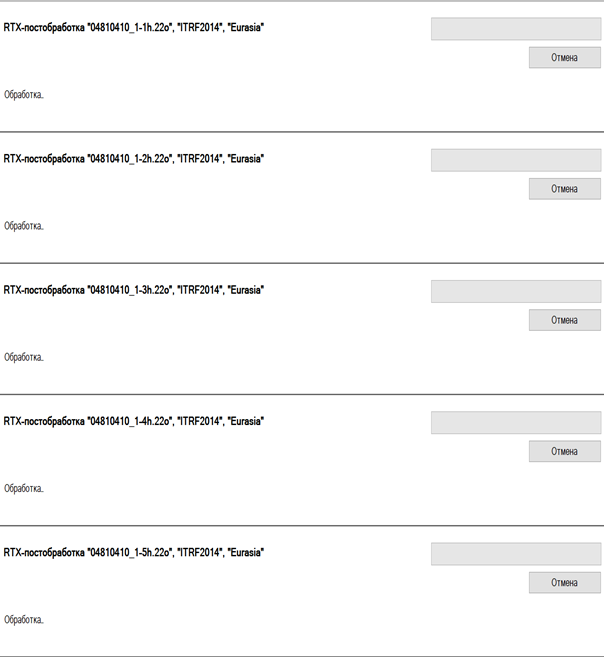
\includegraphics[width=\linewidth]{images/pic10}
	\caption{Обработка в ПО TBC}
	\label{fig:pic10}
\end{figure}

Таким образом была выполнена обработка RINEX файлов продолжительностью  от $\nicefrac{1}{4}$ до $5$ часов ($15, 30, 45$ минут, $1, 2, 3, 4$ и $5$ часов). В таблице~\cref{tab:tab16} приведены разности координат при использовании ПО TBC \cite{mak05,mak08}.


\begin{table} [htbp]
	\centering\small
	\captionof{table}{Влияние продолжительности измерений. ПО TBC }\label{tab:tab16}{%\resizebox{\linewidth}{!}{%
			\begin{tabular}{|c|c|c|c|c|}
				\hline
				\textbf{Продолжительность} & \textbf{σX, м}   & \textbf{σY, м} & \textbf{σZ, м} & $\mathbf{m_{xyz}}$ \\ \hline
				$\nicefrac{1}{4}$ ч        & $0,068$          & $0,073$        & $0,072$        & $0,123$            \\ \hline
				$\nicefrac{1}{2}$ ч        & $0,036$          & $0,052$        & $0,062$        & $0,089$            \\ \hline
				$\nicefrac{3}{4}$ ч        & $0,032$          & $0,036$        & $0,043$        & $0,065$            \\ \hline
				$1$ ч                      & $0,027$          & $0,028$        & $0,035$        & $0,052$            \\ \hline
				$2$ ч                      & $0,025$          & $0,018$        & $0,028$        & $0,042$            \\ \hline
				$3$ ч                      & $0,021$          & $0,017$        & $0,021$        & $0,034$            \\ \hline
				$4$ ч	                   & $0,021$          & $0,017$        & $0,021$        & $0,034$            \\ \hline
				$5$ ч                      & $0,021$          & $0,017$        & $0,021$        & $0,034$            \\ \hline
			\end{tabular}
		}
	\end{table}

На основе данных из таблицы~\cref{tab:tab16} был построен график (рисунок~\cref{fig:pic11}), иллюстрирующий влияние продолжительности измерений на точность определения координат.

\begin{figure}[h]
	\centerfloat{
		\input{images/pic11.tikz}
	}
	\caption{Влияние продолжительности измерений на точность определения координат при обработке в ПО TBC}\label{fig:pic11}
\end{figure}


\subsubsection{Обработка данных с использованием интернет-сервиса APPS }\label{subsec:ch2/sec3/sub2/sub3}

Используя интернет-сервис APPS была выполнена обработка тех же RINEX файлов, что и в предыдущих пунктах. Разности координат приведены в таблице~\cref{tab:tab17}.


\begin{table} [htbp]
	\centering\small
	\captionof{table}{Влияние продолжительности измерений. Сервис APPS }\label{tab:tab17}{%\resizebox{\linewidth}{!}{%
			\begin{tabular}{|c|c|c|c|c|}
				\hline
				\textbf{Продолжительность} & \textbf{σX, м}   & \textbf{σY, м} & \textbf{σZ, м} & $\mathbf{m_{xyz}}$ \\ \hline
				$\nicefrac{1}{4}$ ч        & $-$              & $-$            & $-$            & $-$                \\ \hline
				$\nicefrac{1}{2}$ ч        & $0,102$          & $0,152$        & $0,144$        & $0,233$            \\ \hline
				$\nicefrac{3}{4}$ ч        & $0,093$          & $0,105$        & $0,122$        & $0,186$            \\ \hline
				$1$ ч                      & $0,065$          & $0,076$        & $0,098$        & $0,140$            \\ \hline
				$2$ ч                      & $0,056$          & $0,056$        & $0,068$        & $0,104$            \\ \hline
				$3$ ч                      & $0,048$          & $0,038$        & $0,057$        & $0,084$            \\ \hline
				$4$ ч	                   & $0,048$          & $0,038$        & $0,056$        & $0,083$            \\ \hline
				$5$ ч                      & $0,047$          & $0,038$        & $0,056$        & $0,082$            \\ \hline
			\end{tabular}
		}
	\end{table}


Анализируя таблицу~\cref{tab:tab17} можно заметить, что координаты, определенные при использовании интернет-сервиса APPS, имеют значительно большую величину ошибки в сравнении с другими подходами к обработке. Более того измерения продолжительностью  15~минут вообще нельзя обрабатывать \cite{mak03,mak06}.




\subsubsection{Основные выводы по влиянию продолжительности измерений на получаемые координаты }\label{subsec:ch2/sec3/sub2/sub4}

На основании таблиц и графиков, приведенных в пункте \cref{subsec:ch2/sec3/sub2} можно сделать следующие выводы о влиянии продолжительности измерений на получаемые координаты:

\begin{enumerate}
	\item Точность определения координат практически идентична при использовании большинства интернет-сервисов и программных обеспечений.
	\item Нецелесообразно производить измерения на открытой местности продолжительностью более трёх часов, поскольку точность перестаёт зависеть от продолжительности измерений и остаётся практически неизменной.
	\item На сайтах интернет-сервисов отсутствует информация о минимальном времени необходимом для достижения сходимости решения.
\end{enumerate}




\subsection[Влияние используемых ГНСС и количества спутников]{Исследование влияния различных ГНСС и количества используемых спутников на точность определения координат при использовании РРР-алгоритма}\label{subsec:ch2/sec3/sub3}

С целью исследования влияния различных комбинаций ГНСС на точность определения координат на основе RINEX файлах одного из дней наблюдений ($1, 2, 3, 4$ часов) были получены RINEX файлы, содержащие данные:
\begin{itemize}
	\item только GPS измерения: $(G)$;
	\item только ГЛОНАСС измерения: $(R)$;
	\item комбинацию измерений GPS и ГЛОНАСС: $(G+R)$.
\end{itemize}
В настоящее время отсутствует возможность определения координат только по спутникам ГЛОНАСС, однако можно обрабатывать отдельно GPS и комбинацию спутников ГЛОНАСС\thinspace+\thinspace GPS.

В таблицах \cref{tab:tab18,tab:tab19,tab:tab20} приведены разности координат, полученные при обработке вышеуказанных RINEX-файлов.


\begin{table} [htbp]
	\centering\small
	\captionof{table}{Влияние продолжительности измерений. Сервис CRSR }\label{tab:tab18}{%\resizebox{\linewidth}{!}{%
		\hfill
		\begin{subtable}{.33\linewidth}	
			\centering
			\caption*{\textbf{\textit{GPS}}}
			\begin{tabular}{|c|c|c|c|}
				\hline
				$\mathbf{t}$ \textbf{,ч}   & \textbf{σX, м}    & \textbf{σY, м}  & \textbf{σZ, м} \\ \hline
				$1$ ч                      & $ 0,031$          & $-0,023$        & $-0,025$        \\ \hline
				$2$ ч                      & $ 0,028$          & $-0,019$        & $-0,023$        \\ \hline
				$3$ ч                      & $ 0,023$          & $-0,015$        & $-0,021$        \\ \hline
				$4$ ч	                   & $ 0,023$          & $-0,014$        & $-0,021$        \\ \hline
			\end{tabular}
		\end{subtable}%
		\qquad
		\begin{subtable}{.33\linewidth}	
			\centering
			\caption*{\textbf{\textit{ГЛОНАСС + GPS}}}
			\begin{tabular}{|c|c|c|c|}
				\hline
				$\mathbf{t}$ \textbf{,ч}   & \textbf{σX, м}    & \textbf{σY, м}  & \textbf{σZ, м}  \\ \hline
				$1$ ч                      & $ 0,025$          & $-0,016$        & $-0,020$        \\ \hline
				$2$ ч                      & $ 0,019$          & $-0,012$        & $-0,014$        \\ \hline
				$3$ ч                      & $ 0,016$          & $-0,009$        & $-0,013$        \\ \hline
				$4$ ч	                   & $ 0,016$          & $-0,009$        & $-0,012$        \\ \hline
			\end{tabular}
		\end{subtable}\hfill%
	}
\end{table}


\begin{table} [htbp]
	\centering\small
	\captionof{table}{Влияние продолжительности измерений. Сервис APPS }\label{tab:tab19}{%\resizebox{\linewidth}{!}{%
			\hfill
			\begin{subtable}{.33\linewidth}	
				\centering
				\caption*{\textbf{\textit{GPS}}}
				\begin{tabular}{|c|c|c|c|}
					\hline
					$\mathbf{t}$ \textbf{,ч}   & \textbf{σX, м}    & \textbf{σY, м}  & \textbf{σZ, м}  \\ \hline
					$1$ ч                      & $ 0,041$          & $-0,033$        & $-0,035$        \\ \hline
					$2$ ч                      & $ 0,038$          & $-0,029$        & $-0,028$        \\ \hline
					$3$ ч                      & $ 0,033$          & $-0,025$        & $-0,024$        \\ \hline
					$4$ ч	                   & $ 0,031$          & $-0,023$        & $-0,019$        \\ \hline
				\end{tabular}
			\end{subtable}%
			\qquad
			\begin{subtable}{.33\linewidth}	
				\centering
				\caption*{\textbf{\textit{ГЛОНАСС + GPS}}}
				\begin{tabular}{|c|c|c|c|}
					\hline
					$\mathbf{t}$ \textbf{,ч}   & \textbf{σX, м}    & \textbf{σY, м}  & \textbf{σZ, м}  \\ \hline
					$1$ ч                      & $-0,029$          & $ 0,028$        & $ 0,027$        \\ \hline
					$2$ ч                      & $ 0,025$          & $ 0,024$        & $ 0,025$        \\ \hline
					$3$ ч                      & $-0,024$          & $ 0,019$        & $ 0,019$        \\ \hline
					$4$ ч	                   & $-0,021$          & $ 0,018$        & $ 0,018$        \\ \hline
				\end{tabular}
			\end{subtable}\hfill%
	}
\end{table}
	

\begin{table} [htbp]
	\centering\small
	\captionof{table}{Влияние продолжительности измерений. Сервис Trimble RTX }\label{tab:tab20}{%\resizebox{\linewidth}{!}{%
			\hfill
			\begin{subtable}{.33\linewidth}	
				\centering
				\caption*{\textbf{\textit{GPS}}}
				\begin{tabular}{|c|c|c|c|}
					\hline
					$\mathbf{t}$ \textbf{,ч}   & \textbf{σX, м}    & \textbf{σY, м}  & \textbf{σZ, м} \\ \hline
					$1$ ч                      & $ 0,026$          & $-0,019$        & $-0,025$        \\ \hline
					$2$ ч                      & $-0,019$          & $-0,014$        & $-0,018$        \\ \hline
					$3$ ч                      & $-0,017$          & $-0,012$        & $-0,014$        \\ \hline
					$4$ ч	                   & $-0,017$          & $-0,012$        & $-0,014$        \\ \hline
				\end{tabular}
			\end{subtable}%
			\qquad
			\begin{subtable}{.33\linewidth}	
				\centering
				\caption*{\textbf{\textit{ГЛОНАСС + GPS}}}
				\begin{tabular}{|c|c|c|c|}
					\hline
					$\mathbf{t}$ \textbf{,ч}   & \textbf{σX, м}    & \textbf{σY, м}  & \textbf{σZ, м}  \\ \hline
					$1$ ч                      & $ 0,018$          & $-0,013$        & $-0,020$        \\ \hline
					$2$ ч                      & $-0,013$          & $-0,010$        & $-0,014$        \\ \hline
					$3$ ч                      & $-0,012$          & $-0,008$        & $-0,011$        \\ \hline
					$4$ ч	                   & $-0,012$          & $-0,008$        & $-0,011$        \\ \hline
				\end{tabular}
			\end{subtable}\hfill%
		}
	\end{table}
	
Анализируя таблицы \cref{tab:tab18,tab:tab19,tab:tab20} можно заметить, что точность определения координат при использовании интернет-сервисов CRSR и RTX практически одинакова. 
На примере интернет-сервиса Trimble RTX при сравнении разностей координат, полученных при обработке различных комбинаций ГНСС, установлено повышение точности определения координат: X и Y на 30\%, Z --- на 20\% \cite{mak01,src83,src88,src89}.
Также было установлено, что использование дополнительных систем ГНСС (BeiDou, Galileo) не повышает точность определения координат.

В дополнение была выполнена косвенная оценка влияния pdop фактора. В таблице \cref{tab:tab21} приводятся численные значения количества используемых спутников и изменение pdop.

\begin{table} [htbp]
	\centering\small
%	\begin{threeparttable}% выравнивание подписи по границам таблицы
		\captionof{table}{Зависимость p-dop от количества спутников. Сервис Trimble RTX }
		\label{tab:tab21}{%\resizebox{\linewidth}{!}{%
%			\hfill
			\begin{subtable}{.37\linewidth}	
				\centering
				\caption*{\textbf{\textit{GPS}}}
				\begin{tabular}{|c|c|c|c|}
					\hline
					$\mathbf{T_\text{изм.}}$	&$\mathbf{p-dop_{min}}$	&$\mathbf{p-dop_{max}}$	& $\mathbf{N}$ \\ \hline
					$1$ ч						& $ 1,38$				& $ 2,07$        		& $ 12$   \\ \hline
					$2$ ч						& $ 1,38$				& $ 2,13$        		& $ 14$   \\ \hline
					$3$ ч						& $ 1,38$				& $ 2,59$        		& $ 16$   \\ \hline
					$4$ ч						& $ 1,50$          		& $ 3,57$        		& $ 19$   \\ \hline
				\end{tabular}
			\end{subtable}%
			\qquad
			\begin{subtable}{.57\linewidth}	
				\centering
				\caption*{\textbf{\textit{ГЛОНАСС + GPS}}}
				\begin{tabular}{|c|c|c|c|}
					\hline
					$\mathbf{T_\text{изм.}}$	&$\mathbf{p-dop_{min}}$	&$\mathbf{p-dop_{max}}$	& $\mathbf{N}$	\\ \hline
					$1$ ч						& $ 1,27$				& $ 1,73$        		& $ 19(12+7)$	\\ \hline
					$2$ ч						& $ 1,27$				& $ 1,73$        		& $ 23(14+9)$	\\ \hline
					$3$ ч						& $ 1,21$				& $ 1,84$        		& $ 26(16+10)$	\\ \hline
					$4$ ч						& $ 1,21$          		& $ 2,19$        		& $ 30(19+11)$	\\ \hline
				\end{tabular}
			\end{subtable}%\hfill%
			\legend{\small
				$\mathbf{T_\text{изм.}}$ --~ продолжительность измерений,\enspace
				$\mathbf{N}$ --~ количество спутников \textbf{Всего\thinspace (GPS\thinspace +\thinspace ГЛОНАСС)},\newline
				\thinspace$\mathbf{p-dop_{min}}$ --~ минимальный \textbf{p-dop},\enspace
				$\mathbf{p-dop_{max}}$ --~  максимальный \textbf{p-dop}.
			}
		}
%		\end{threeparttable}
	\end{table}
	
На рисунках \cref{fig:pic12,fig:pic13,fig:pic14,fig:pic15,fig:pic16,fig:pic17,fig:pic18,fig:pic19} приведены графики изменения PDOP в зависимости от ГНСС и продолжительности измерений.	


\begin{figure}[!h]
	\centering
	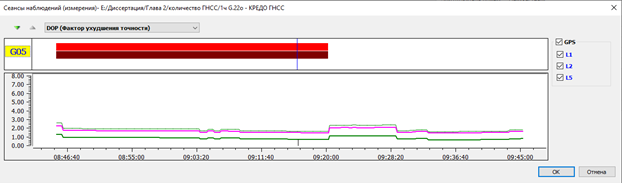
\includegraphics[width=0.99\linewidth]{images/pic12}
	\caption{Изменение p-dop фактора. ГНСС: GPS. $T_{\text{изм.}}=1$ ч. }
	\label{fig:pic12}
\end{figure}

\begin{figure}[!h]
	\centering
	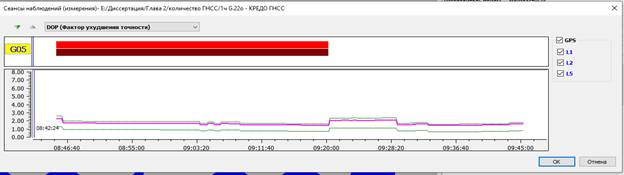
\includegraphics[width=0.99\linewidth]{images/pic13}
	\caption{Изменение p-dop фактора. ГНСС: ГЛОНАСС\thinspace +\thinspace GPS. $T_{\text{изм.}}=1$ ч. }
	\label{fig:pic13}
\end{figure}

\begin{figure}[!h]
	\centering
	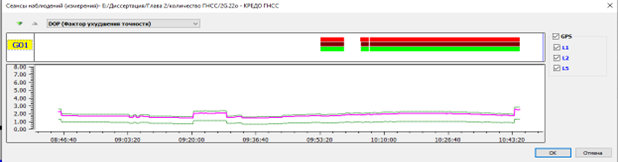
\includegraphics[width=0.99\linewidth]{images/pic14}
	\caption{Изменение p-dop фактора. ГНСС: GPS. $T_{\text{изм.}}=2$ ч. }
	\label{fig:pic14}
\end{figure}

\begin{figure}[!h]
	\centering
	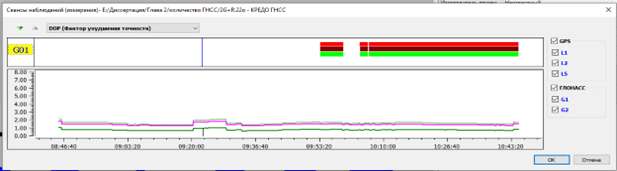
\includegraphics[width=0.99\linewidth]{images/pic15}
	\caption{Изменение p-dop фактора. ГНСС: ГЛОНАСС\thinspace +\thinspace GPS. $T_{\text{изм.}}=2$ ч. }
	\label{fig:pic15}
\end{figure}

\begin{figure}[!h]
	\centering
	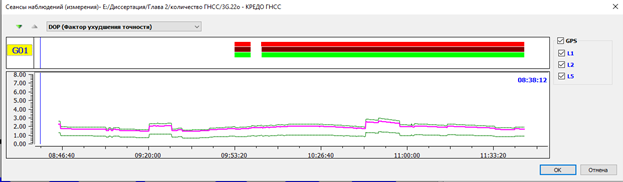
\includegraphics[width=0.99\linewidth]{images/pic16}
	\caption{Изменение p-dop фактора. ГНСС: GPS. $T_{\text{изм.}}=3$ ч. }
	\label{fig:pic16}
\end{figure}

\begin{figure}[!h]
	\centering
	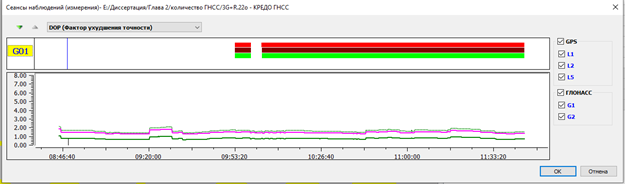
\includegraphics[width=0.99\linewidth]{images/pic17}
	\caption{Изменение p-dop фактора. ГНСС: ГЛОНАСС\thinspace +\thinspace GPS. $T_{\text{изм.}}=3$ ч. }
	\label{fig:pic17}
\end{figure}

\begin{figure}[!h]
	\centering
	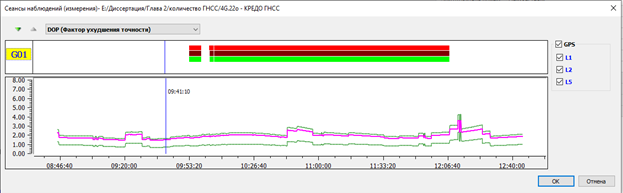
\includegraphics[width=0.99\linewidth]{images/pic18}
	\caption{Изменение p-dop фактора. ГНСС: GPS. $T_{\text{изм.}}=4$ ч. }
	\label{fig:pic18}
\end{figure}

\begin{figure}[!h]
	\centering
	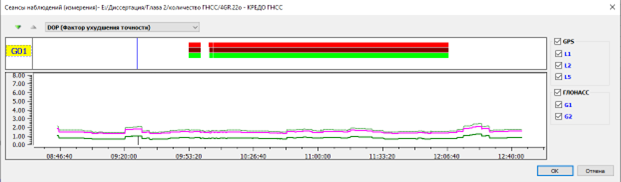
\includegraphics[width=0.99\linewidth]{images/pic19}
	\caption{Изменение p-dop фактора. ГНСС: ГЛОНАСС\thinspace +\thinspace GPS. $T_{\text{изм.}}=4$ ч. }
	\label{fig:pic19}
\end{figure}
	
С целью исследования влияния количества спутников на получаемую точность определения координат была написана программа \texttt{rinmix} на языке программирования \texttt{python}. На рисунке \cref{fig:pic20} приведен экран с описанием управляющих параметров командной строки для данной программы.

\begin{figure}[!h]
	\centering
	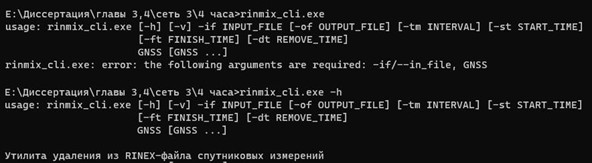
\includegraphics[width=0.99\linewidth]{images/pic20}
	\caption{Управляющие параметры командной строки программы rinmix }
	\label{fig:pic20}
\end{figure}

Для осуществления редактирования программе указывается путь к редактируемому RINEX-файлу и номера удаляемых спутников. Опционально можно указать параметры времени удаляемого интервала и путь к выходному файлу. Отфильтрованный RINEX-файл по умолчанию располагается в той же папке, что и исходный.

С помощью данной программы была проведена фильтрация RINEX-файлов и были получены файлы содержащие: $40, 35, 30, 25, 20, 15, 10, 8, 5$ спутников. После этого была выполнена их обработка, в результате которой были определены 15 векторов. Впоследствии были найдены разности приращений координат (вычисленных и эталонных), приведённые в таблице \cref{tab:tab22}.

\begin{table} [htbp]
	\centering\small
	\captionof{table}{Зависимость точности от pdop-фактора и количества спутников }\label{tab:tab22}{%
			\begin{tabular}{|c|c|c|c|c|c|c|c|c|}
				\hline
				$\mathbf{N_\text{спутн.}}$ & \textbf{35} & \textbf{30} & \textbf{25} & \textbf{20} & \textbf{15} & \textbf{10} & \textbf{8} & \textbf{5} \\ \hline
				\textbf{p-dop}	& 0,99   & 1,02   & 1,25   & 1,45   & 1,68   & 2,15   & 2,42   & 2,62   \\ \hline
				\textbf{ГНСС}	& G+R+E  & G+R+E  & G+R+E  & G+R+E  & G+R    & G+R    & G+R    & G+R    \\ \hline
				\textbf{δX, м}	& 0,010  & 0,011  & 0,011  & 0,018  & 0,019  & 0,029  & 0,035  & 0,075  \\ \hline
				\textbf{δY, м}	& -0,004 & -0,005 & -0,006 & -0,006 & -0,016 & -0,021 & -0,035 & -0,086 \\ \hline
				\textbf{δZ, м}	& 0,012  & 0,012  & 0,013  & 0,013  & 0,015  & 0,019  & 0,036  & 0,063  \\ \hline
				\textbf{δS, м}	& 0,011  & 0,010  & 0,011  & 0,018  & 0,019  & 0,029  & 0,035  & 0,075  \\ \hline
			\end{tabular}
	}
\end{table}

При анализе данной таблицы можно заметить, что точность практически неизменна при использовании в обработке 15 спутников и больше. На рисунках \cref{fig:pic21,fig:pic22,fig:pic23,fig:pic24} 21,22,23,24 приведены результаты в графическом виде.


\begin{figure}[h]
	\centerfloat{
		\input{images/pic21.tikz}
	}
	\caption{Влияние количества спутников на точность по оси X}\label{fig:pic21}
\end{figure}

\begin{figure}[h]
	\centerfloat{
		\input{images/pic22.tikz}
	}
	\caption{Влияние количества спутников на точность по оси Y}\label{fig:pic22}
\end{figure}

\begin{figure}[h]
	\centerfloat{
		\input{images/pic23.tikz}
	}
	\caption{Влияние количества спутников на точность по оси Z}\label{fig:pic23}
\end{figure}

\begin{figure}[h]
	\centerfloat{
		\input{images/pic24.tikz}
	}
	\caption{Влияние количества спутников на точность σS}\label{fig:pic24}
\end{figure}


\subsubsection{Основные выводы по влиянию конфигураций ГНСС и количества спутников на получаемую точность определения координат }\label{subsec:ch2/sec3/sub3/sub1}

\begin{enumerate}
	\item Отсутствует возможность обработки данных только ГЛОНАСС.
	\item Точность определения координат при обработке RINEX-файлов, содержащих только GPS и совместной обработки спутников GPS и ГЛОНАСС при одиночном позиционировании практически неизменна при 1 часе и выше.
	\item При увеличении длительности измерений свыше одного часа точность определения координат улучшается на 3--4 см.
	\item При увеличении количества спутников в обработке свыше 15 точность остаётся практически неизменной. P-dop фактор оказывает влияние на получаемые точности. 
\end{enumerate}



\subsection{Влияние дискретности данных на получаемую точность}\label{subsec:ch2/sec3/sub4}


С целью исследования влияния дискретности на точность определения координат по РРР-алгоритму была взята выбора из массива данных с частотой записи $1, 5, 10, 20, 30$ секунд. Данные были обработаны с использованием интернет-сервиса Trimble RTX.

В таблице \cref{tab:tab23} на странице\footnote{Помимо ссылок на объекты (таблицы, формулы, рисунки, вообще всё, что мы отмечаем в тексе метками) мы можем указывать автоматически вычисляемые номера страниц, где они расположены.} \pageref{tab:tab23} приводятся результаты разностей векторов.



\begin{table} [htbp]
	\centering\small
	\captionof{table}{Влияние частоты записи на точность определения координат. Сервис Trimble RTX\tnote{0} }\label{tab:tab23}{
			\hfill
			\begin{subtable}{.47\linewidth}	
				\centering
				\caption{$\mathbf{t_\text{изм.}=1\text{, ч}}$}
				\begin{tabular}{|c|c|c|c|}
					\hline
					\textbf{Интервал, с}	& \textbf{δdX, м}	& \textbf{δdY, м}	& \textbf{δdZ, м}	\\ \hline
					$ 1$					& $-0,011$			& $-0,010$			& $ 0,005$			\\ \hline
					$ 5$					& $-0,011$			& $-0,010$			& $ 0,005$			\\ \hline
					$10$					& $-0,010$			& $-0,011$			& $ 0,004$			\\ \hline
					$20$					& $-0,012$			& $-0,010$			& $ 0,006$			\\ \hline
					$30$					& $-0,011$			& $-0,009$			& $ 0,004$			\\ \hline
				\end{tabular}
			\end{subtable}%
			\qquad
			\begin{subtable}{.47\linewidth}	
				\centering
				\caption{$\mathbf{t_\text{изм.}=2\text{, ч}}$}
				\begin{tabular}{|c|c|c|c|}
					\hline
					\textbf{Интервал, с}	& \textbf{δdX, м}	& \textbf{δdY, м}	& \textbf{δdZ, м}	\\ \hline
					$ 1$					& $-0,003$			& $ 0,002$			& $-0,001$			\\ \hline
					$ 5$					& $-0,003$			& $ 0,002$			& $-0,001$			\\ \hline
					$10$					& $-0,003$			& $ 0,002$			& $-0,001$			\\ \hline
					$20$					& $-0,003$			& $ 0,002$			& $-0,001$			\\ \hline
					$30$					& $-0,003$			& $ 0,002$			& $-0,001$			\\ \hline
				\end{tabular}
			\end{subtable}\hfill%
			
			\hfill
\begin{subtable}{.47\linewidth}	
	\centering
	\caption*{$\mathbf{t_\text{изм.}=1\text{, ч}}$}
	\begin{tabular}{|c|c|c|c|}
		\hline
		\textbf{Интервал, с}	& \textbf{δdX, м}	& \textbf{δdY, м}	& \textbf{δdZ, м}	\\ \hline
		$ 1$					& $-0,011$			& $-0,010$			& $ 0,005$			\\ \hline
		$ 5$					& $-0,011$			& $-0,010$			& $ 0,005$			\\ \hline
		$10$					& $-0,010$			& $-0,011$			& $ 0,004$			\\ \hline
		$20$					& $-0,012$			& $-0,010$			& $ 0,006$			\\ \hline
		$30$					& $-0,011$			& $-0,009$			& $ 0,004$			\\ \hline
	\end{tabular}
\end{subtable}%
\qquad
\begin{subtable}{.47\linewidth}	
	\centering
	\caption*{ж) $\mathbf{t_\text{изм.}=2\text{, ч}}$}
	\begin{tabular}{|c|c|c|c|}
		\hline
		\textbf{Интервал, с}	& \textbf{δdX, м}	& \textbf{δdY, м}	& \textbf{δdZ, м}	\\ \hline
		$ 1$					& $-0,003$			& $ 0,002$			& $-0,001$			\\ \hline
		$ 5$					& $-0,003$			& $ 0,002$			& $-0,001$			\\ \hline
		$10$					& $-0,003$			& $ 0,002$			& $-0,001$			\\ \hline
		$20$					& $-0,003$			& $ 0,002$			& $-0,001$			\\ \hline
		$30$					& $-0,003$			& $ 0,002$			& $-0,001$			\\ \hline
	\end{tabular}
\end{subtable}\hfill%

			
			
			
			
	\begin{tablenotes}
		\item [0] С названиями <<подтаблиц>> можно поступать разными способами:
		\begin{itemize}
			\item можем вставлять с автоматической нумерацией,
			\item но в этом случае, если не лезть глубоко в настройки, нумерация идёт латиницей...
			\item можем вставить без нумерации; 
			\item можем ещё <<закостылить>> и просто руками вставить буквы (или цифры) ;).
		\end{itemize}
		
		\item [1] В любом случае, эти заголовки не появятся ни в списке таблиц, ни в оглавлении.
	\end{tablenotes}
	}
\end{table}

Из таблицы видно, что при уменьшении частоты записи до 60 секунд точность определения координат начинает ухудшаться.

\begin{quote}
	Вообще-то из таблицы этого не видно, т.к. во-первых, в ней нет интервалов больше $30$~секунд, а во-вторых, там вообще нет статистически значимых изменений в зависимости от частоты записи... :(
\end{quote}


\subsection{$\ldots$}\label{subsec:ch2/sec3/sub5}

235


\section{Заключение по главе}\label{sec:ch2/sect4}

Целью второй главы данной диссертационной работы являлось провести исследование точности определения координат одиночного спутникового позиционирования при обработке по РРР-алгоритму. В качестве оцениваемых факторов были выбраны следующие:
\begin{enumerate}
	\item Продолжительность измерений.
	\item Количество ГНСС.
	\item Количество используемых спутников для обработки данных.
	\item Дискретность данных.
	\item Проведение многократных спутниковых измерений.
	\item Влияния тех или иных способов и методов.
\end{enumerate}
Ниже представлены основные подвыводы по каждому из пунктов.

\subsection*{Продолжительность измерений}\label{subsec:ch2/sec4/sub-1}

В результате исследований было выявлено, что точность определения координат при использовании спутниковых методов позиционирования для создания геодезических сетей неизменна при 2-х часах и выше. При 3-х часах и более точность практически неизменна, а максимальная величина изменения составляет несколько мм. Исходя из этого можно сделать вывод, что проводить измерения более 3-х часов фактически нецелесообразно.

\subsection*{Сравнение подходов к обработке данных по РРР-алгоритму}\label{subsec:ch2/sec4/sub-2}

В настоящее время существуют различные способы обработки данных по РРР-алгоритму. В Работе сделан акцент на использование этих методов обработки:
\begin{itemize}
	\item коммерческие программные обеспечения (TBC);
	\item интернет-сервисы (RTX, CRSR, APPS, AUSPOS).
\end{itemize}
По результатам выполнения работ установлено, что точность определения координат при использовании коммерческих программных обеспечений и большинства интернет-сервисов практически совпадает. Точность получения координат при использовании интернет-сервиса \textbf{AUSPOS, APPS. GAPS} значительно ниже, чем при использовании остальных интернет-сервисов.

\subsection*{Влияние дискретности данных}\label{subsec:ch2/sec4/sub-3}

При снижении частоты записи до 60 секунд точность определения координат падает.

\subsection*{Исследование точности определения координат при многократных спутниковых измерениях}\label{subsec:ch2/sec4/sub-4}

В зависимости от выбранного интернет-сервиса несколько варьируется точность определения координат. В сравнении сервисов RTX и CRSR обеспечивается примерно одинаковая точность определения координат (в среднем 2,5\thinspace см при 1 часе по оси Х. по остальным осям точность несколько выше).

\subsection*{Влияние различных комбинаций ГНСС}\label{subsec:ch2/sec4/sub-5}

Выполнено сравнение точности определения координат при использовании 2-х наборов ГНСС, содержащих: только данные GPS (G) и GPS совместно с ГЛОНАСС (G+R). По результатам эксперимента можно сделать вывод, что точность определения координат при обработке данных G+R выше в среднем на 30\%, чем при определении координат только при G.

\subsection*{Влияние количества принимаемых спутников}\label{subsec:ch2/sec4/sub-6}

При использовании 15 спутников и выше точность определения координат практически неизменна. При меньшем количестве спутников точность заметно падает. Pdop-фактор оказывает значительное влияние на получаемую точность.


\textbf{\textit{КОНЕЦ ВТОРОЙ ГЛАВЫ}}\footnote{Требуется вычитать, исправить и существенно переписать выводы по главе. }

